\label{sec:design}

Libraries such as Embree (section~\ref{sec:embree}) provide optimized ray 
tracing algorithms that exploit parallelism on a single machine.  When we look
at larger data sets that will no longer fit into the memory of a single machine,
we may consider the use of distributed systems, see section~\ref{sec:computing},
to render images.  The next generation of distributed systems capable of 
exascale computation provides an opportunity and in some cases a necessity to 
redesign current distributed applications.  Two of the main differences that 
will set exascale systems apart from current distributed systems are the 
increase in the number of nodes available and the reduction of the memory 
available per node.  For algorithm designers, this means there will be increased
communication overhead as data will need to be passed more frequently between 
individual nodes.

Communication-avoiding algorithms have been proposed as a way to reduce 
communication overhead.  The basic idea is to re-do computation instead of 
communicating results.  We use this idea as a basis for designing a distributed 
ray tracing application.  On-node parallelism can be exploited by taking 
advantage of Embree or another optimized library.  This leaves the key challenge 
as how to reduce the communication necessary between the nodes of the 
distributed system.

\section{Data Decomposition}
\label{sec:data_decomposition}
Designing a ray tracer for exascale systems becomes an interesting problem once
we consider scenes to render that have too much information to fit entirely into
the memory of a single node.  In these scenes, some type of data decomposition 
is required where the scene is divided into smaller pieces and distributed 
amongst the available nodes. To fully utilize the on node parallelism we would 
want to give each node enough data to fill its available memory. As each scene 
to be rendered is unique the idealized distribution for one scene will not be 
the same as the idealized distribution for another.  In order to split the data
into equally-sized subsets, a technique known as load balancing is used.

Load balancing is often addressed with a pre-processing step where the domain is 
optimally divided into evenly sized subsets of data before ray tracing beings. 
As the pre-processing step is often computationally expensive, the expense must 
be considered and weighed against alternative designs. For example, a naive 
alternative approach is to divide the space based on a uniform spatial 
distribution.  This results in unevenly balanced subsets of data but takes 
little time to compute.  In this naive approach where the scene has not been 
balanced it is likely to end up with nodes that have lots of work while other 
nodes have little work.

Determining the optimal design pattern for data decomposition becomes a question
of whether the cost of pre-processing outweighs the cost of an unbalanced 
system.  Assuming the pre-processing step were free, computationally speaking, 
the solution would then be to use it.  This would ensure the minimum number of
nodes are used and that each one is used to its full potential, memory wise.  
However since there is a cost to pre-processing we must consider algorithms that
reduce this cost.  

Dividing the domain uniformly in space, for example, reduces the pre-processing 
cost but requires the use of more nodes than would be needed by a load-balanced
distribution.  In addition, each node may or may not fill the memory available. 
Since each node need not be responsible for a single subset of the domain, it is 
possible to offset this concern and increase memory usage per node by assigning 
each node multiple subsets of data.

\begin{figure}[!htb]
\centering
  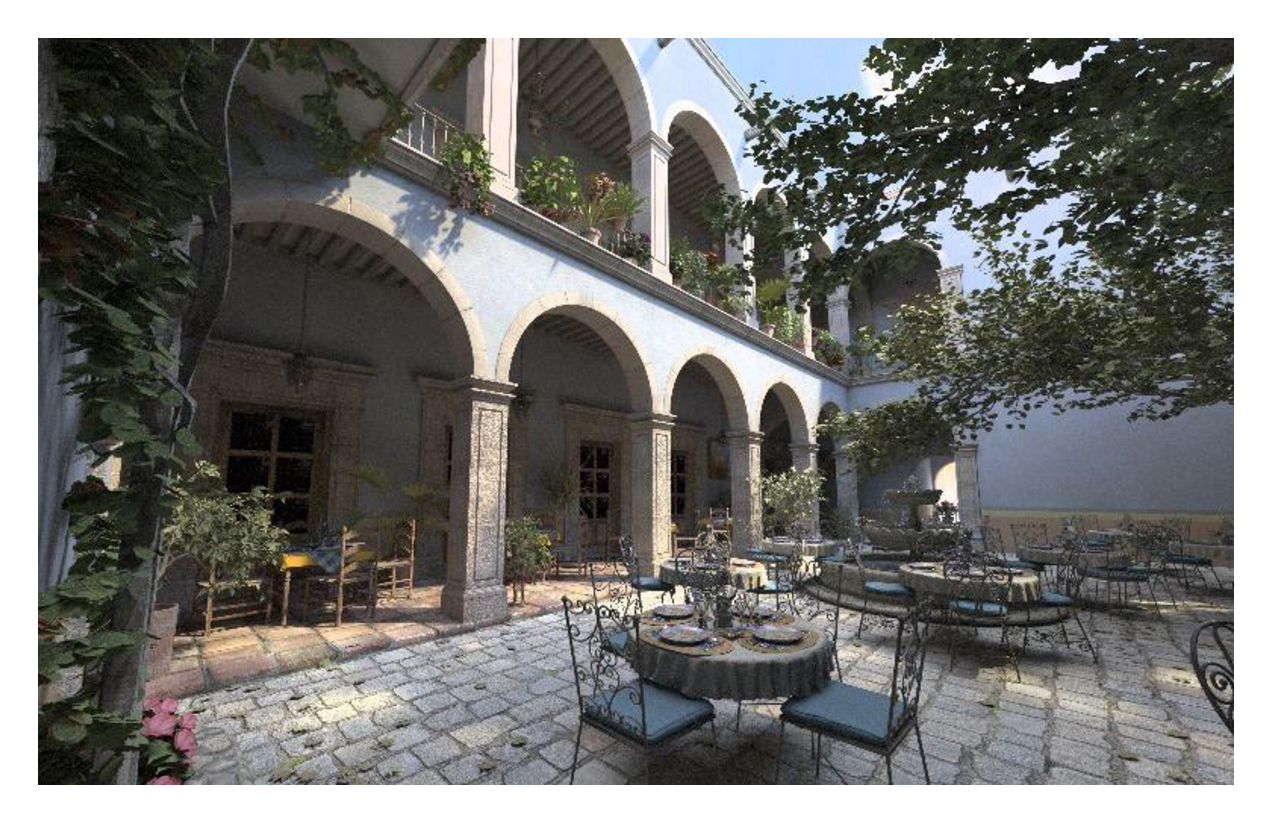
\includegraphics[height=5cm]{drawings/sanmiguel_cam25.pdf}
\caption{San Miguel example scene}
\label{fig:san_miguel}
\end{figure}

As an example we will consider the San Miguel data set, see 
figure~\ref{fig:san_miguel}\footnote{http://www.pbrt.org/scenes\_images/sanmiguel\_cam25.jpg}.  
The scene was modeled by Guillermo M. Leal Llaguno
and is based on a hacienda located in San Miguel de Allende, Mexico.  It is a 
large scene with a nonuniform data distribution.  If we decompose the domain 
into 27 (=3x3x3) equally-sized voxels, we get the distribution shown in 
figure~\ref{fig:san_miguel_data} a.  If we consider ray tracing this scene on a
machine with eight cores, we might get a distribution such as that shown
in figure~\ref{fig:san_miguel_data} b.   This roughly distributes the data 
evenly between the nodes, giving us a setup similar to what a pre-processing 
step designed to optimally distribute the data may compute.  For simplicity we 
will use the spatially uniform data distribution algorithm and focus on reducing 
communication cost.

\begin{figure}[!htb]
\minipage{0.52\textwidth}
  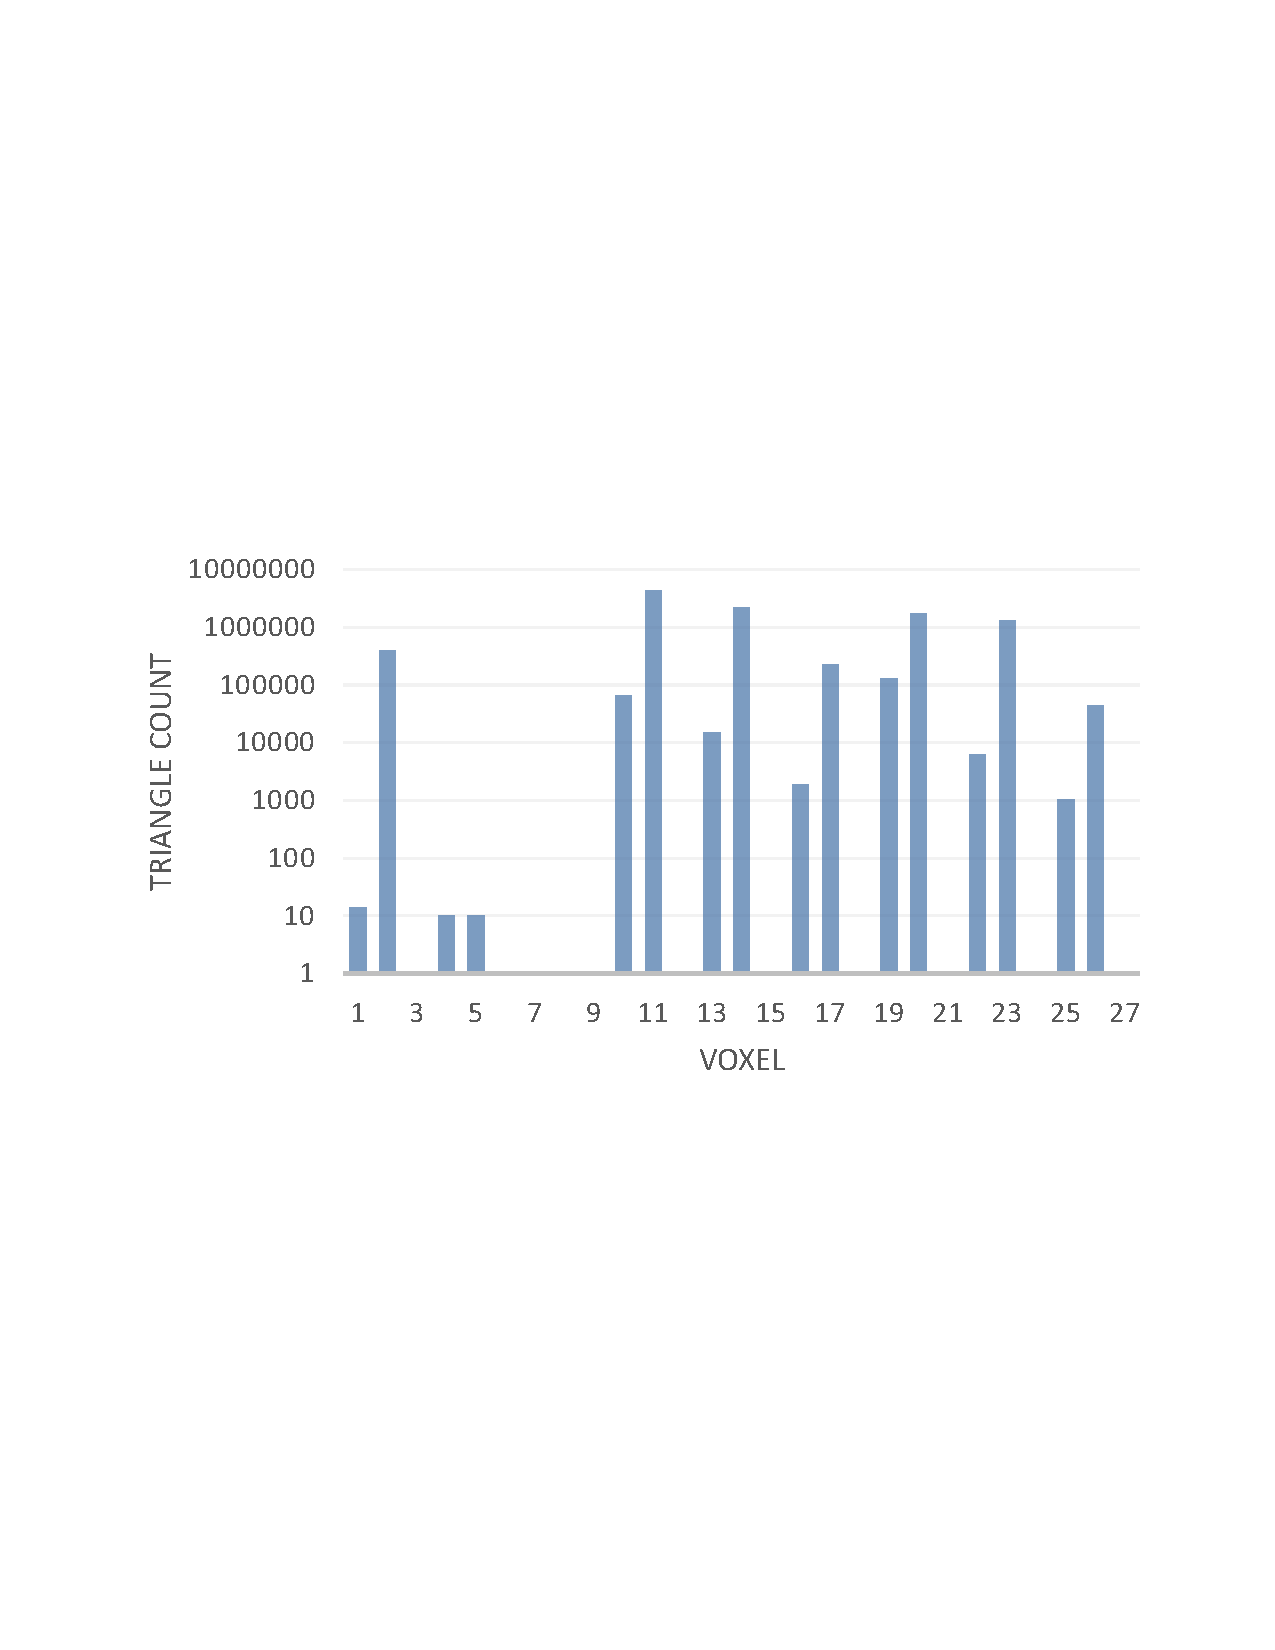
\includegraphics[height=3.8cm]{drawings/VoxelDistribution.pdf}
  
  (a) Triangles per voxel
  
  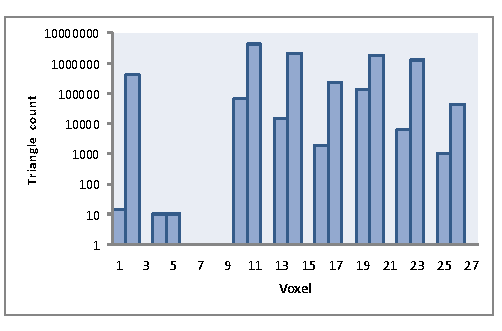
\includegraphics[height=3.8cm]{drawings/DataDistribution.pdf}
  
  (c) Triangles per node  
\endminipage\hfill
\minipage{0.48\textwidth}
  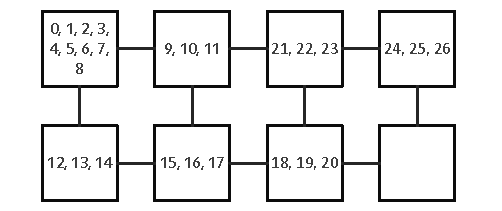
\includegraphics[width=\linewidth]{drawings/NodeDistribution.pdf}  
  
  (b) Node distribution  
\endminipage
\caption{San Miguel data decomposition example}
\label{fig:san_miguel_data}
\end{figure}


\section{Communication} 
\label{sec:communication}
Each ray cast into a scene has the potential to interact with every geometric
shape in the scene due to reflection and refraction\footnote{ %
  Typically a maximum threshold is set to limit the number of times a ray
  can be reflected. 
}.  In addition, each point being illuminated within a scene needs to cast 
secondary rays towards the lights.  These means determining which pieces of 
memory each ray will need throughout the ray tracing algorithm is not a straight
forward task.  With a distributed system and in a worst case scenario, each ray 
may need to communicate with every node.  

Communication is anticipated to be the bottleneck on an exascale system which
makes reducing communication cost high priority in our algorithm design.  
Optimally our goal is to create a ray tracing algorithm with distributed data 
that needs little to no communication.  We explore how we might design a 
communication avoiding ray tracer in this section.

\subsection{Communication-avoiding ray casting}
\label{sec:ca-ray-casting}
To design a communication avoiding ray tracer we will start with a simple ray
casting algorithm where only the viewing rays are traced. These rays are 
cast into a scene from the eye position.  If they intersect with an object, the 
ambient-specular-diffuse color is computed.  Without reflection, refraction and 
secondary rays, communication between nodes executing the ray tracer can be 
avoided entirely.

\begin{figure}[!htb]
\minipage{0.4\textwidth}
\begin{algorithm}
TRACE_RAYS(voxels) 
  in: process for each voxel of 
      data, sorted back to front
  out: image, a ray traced scene
  rays = COMPUTE_PRIMARY_RAYS()
  image[][]
  for all voxel in voxels do
    rays_ = COPY(rays)
    image_ = voxel.TRACE_VOXEL_RAYS(rays_)
    for all x in image.width do
      for all y in image.height do
        if image_[x][y] then
          image[x][y] = image_[x][y];
        end if
      end for
    end for
  end for
return image
\end{algorithm}

(a) Controller code

\endminipage\hfill
\minipage{0.4\textwidth}
\begin{algorithm}
TRACE_VOXEL_RAYS(rays)
  in:  all primary rays
  out: image, a traced scene 
       for this voxel
  image[][]
  for all ray in rays do
    if ray intersects scene then
      image[ray.x][ray.y] = COMPUTE_COLOR(ray)
    else
      image[ray.x][ray.y] = FALSE
    end if
  end for
return rays




.
\end{algorithm}

(b) Per voxel code

\endminipage\hfill
\caption{Ray casting pseudo code}
\label{fig:ray_caster}
\end{figure}

We can avoid all communication between nodes in a ray casting algorithm by 
preemptively sending every ray to every node, see figure~\ref{fig:ray_caster} a.  
Each process executing over a subset of data will receive every viewing ray, see 
figure~\ref{fig:ray_caster} b.  Each process then traces the rays and computes a
color if the ray intersected an object within its data.  

\begin{figure}[!htb]
\minipage{0.5\textwidth}
  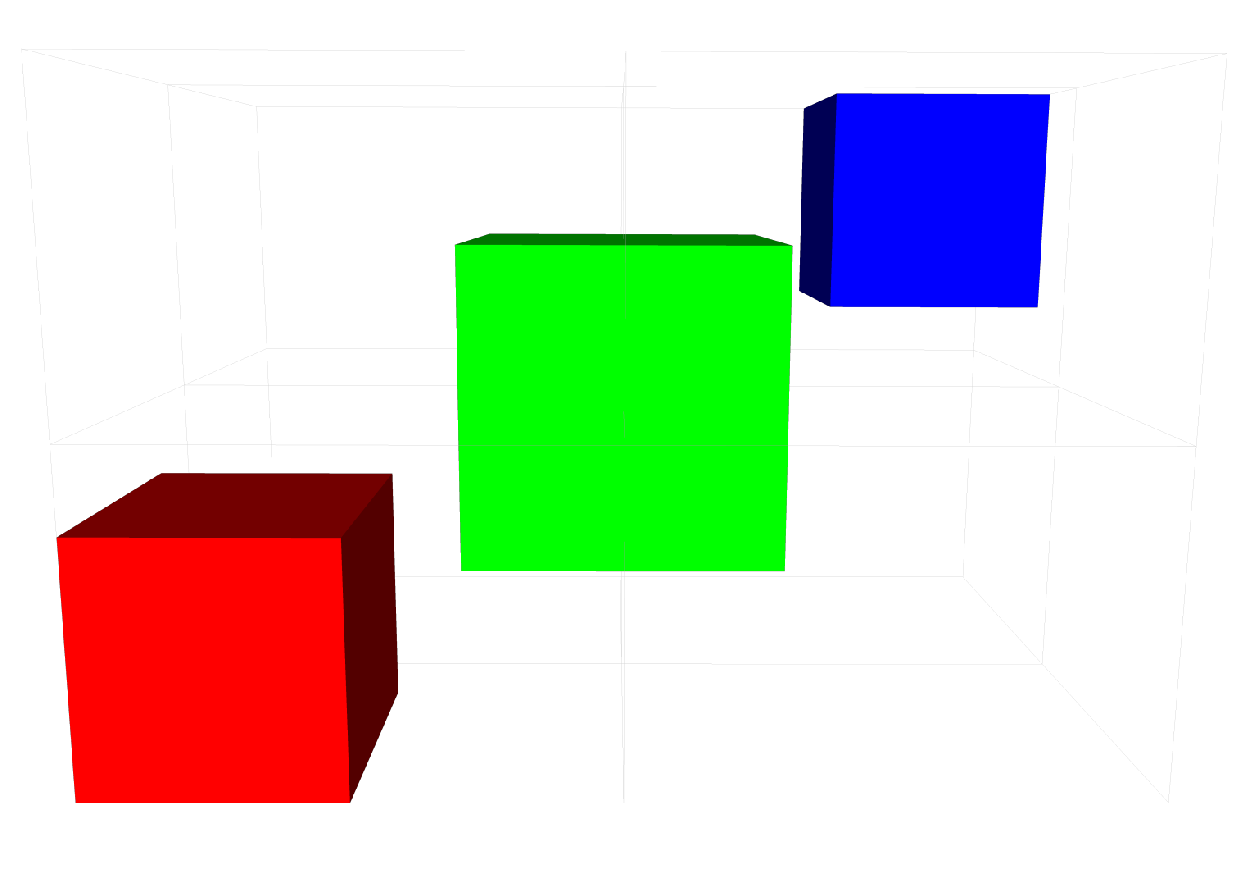
\includegraphics[width=\linewidth]{drawings/side.pdf}
  
(a) Side

\endminipage\hfill
\minipage{0.5\textwidth}
  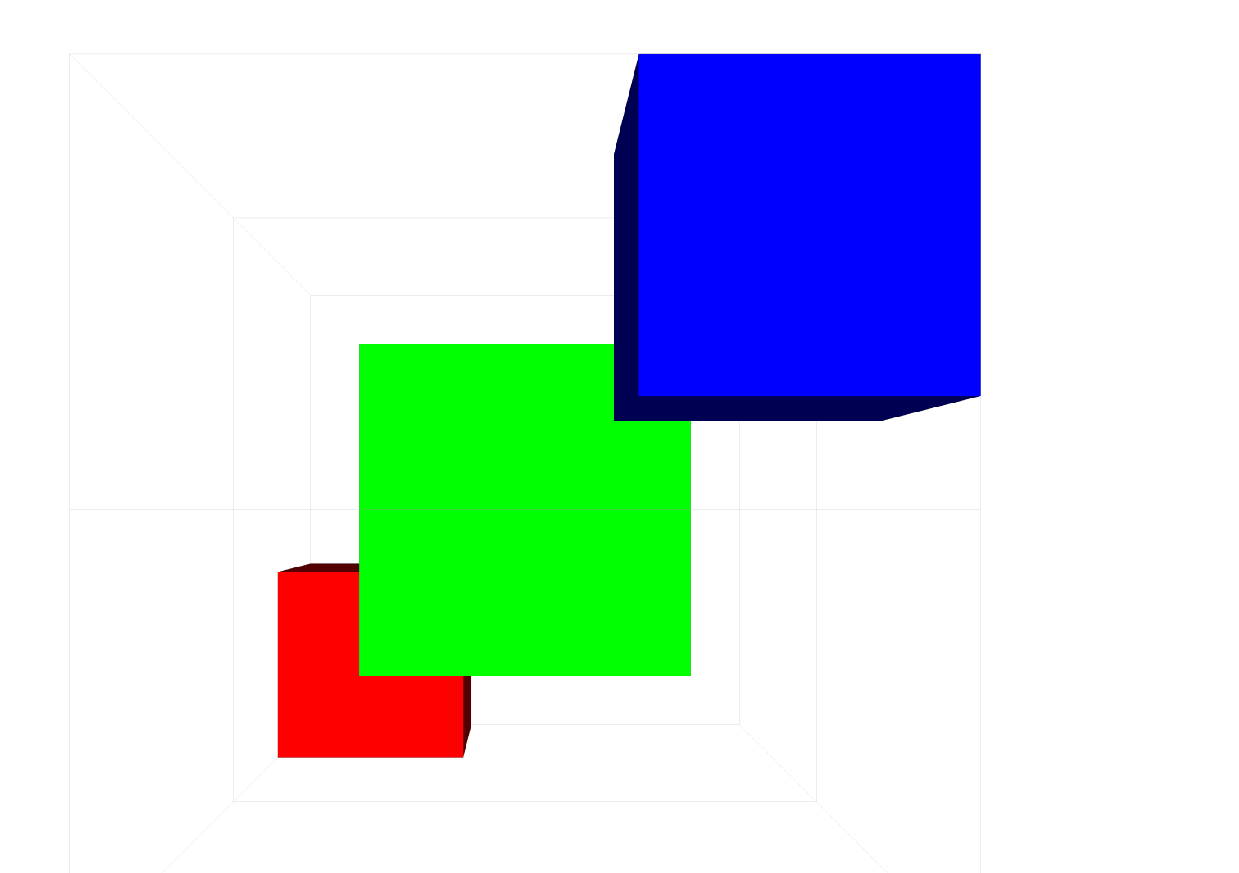
\includegraphics[width=\linewidth]{drawings/front.pdf}
  
(b) Front

\endminipage\hfill
\caption{3D view of example cubes}
\label{fig:cubes_3d}
\end{figure}

The traced rays can then be used to produce the final image using a back to 
front voxel ordering to ensure correct image composition.  As an illustration we 
can consider a simple scene with three cubes placed along a diagonal, 
see figure~\ref{fig:cubes_3d}.  Each cube is broken into twelve triangles, two 
for each face.  If we distribute the data into 8 (=2x2x2) equally-sized subsets
we get eight voxels sharing the green cube, one voxel with the red cube and one 
voxelw ith the blue cube.  The voxels are ordered front to back, bottom to top, 
and left to right, which makes voxel 1 the front bottom left, voxel 2 the front 
bottom right, and voxel 8 the back top right. 

If we trace the scene from the camera view shown in figure~\ref{fig:cubes_3d} b, 
each voxel computation will produce corresponding image shown in 
figure~\ref{fig:cubes}.  The gray in the images are \emph{not} produced by the
computation, they illustrate the extents of the geometry contained by the voxel 
and are there only for clarity.  The dark green in voxels five through eight 
illustrate the voxel tracing the inside of the green cube.  The final image is 
produced, see figure~\ref{fig:cubes_final}, by composing the eight voxel images
started with voxel eight and working back towards voxel one.  

\begin{figure}[!htb]
\minipage{0.25\textwidth}
  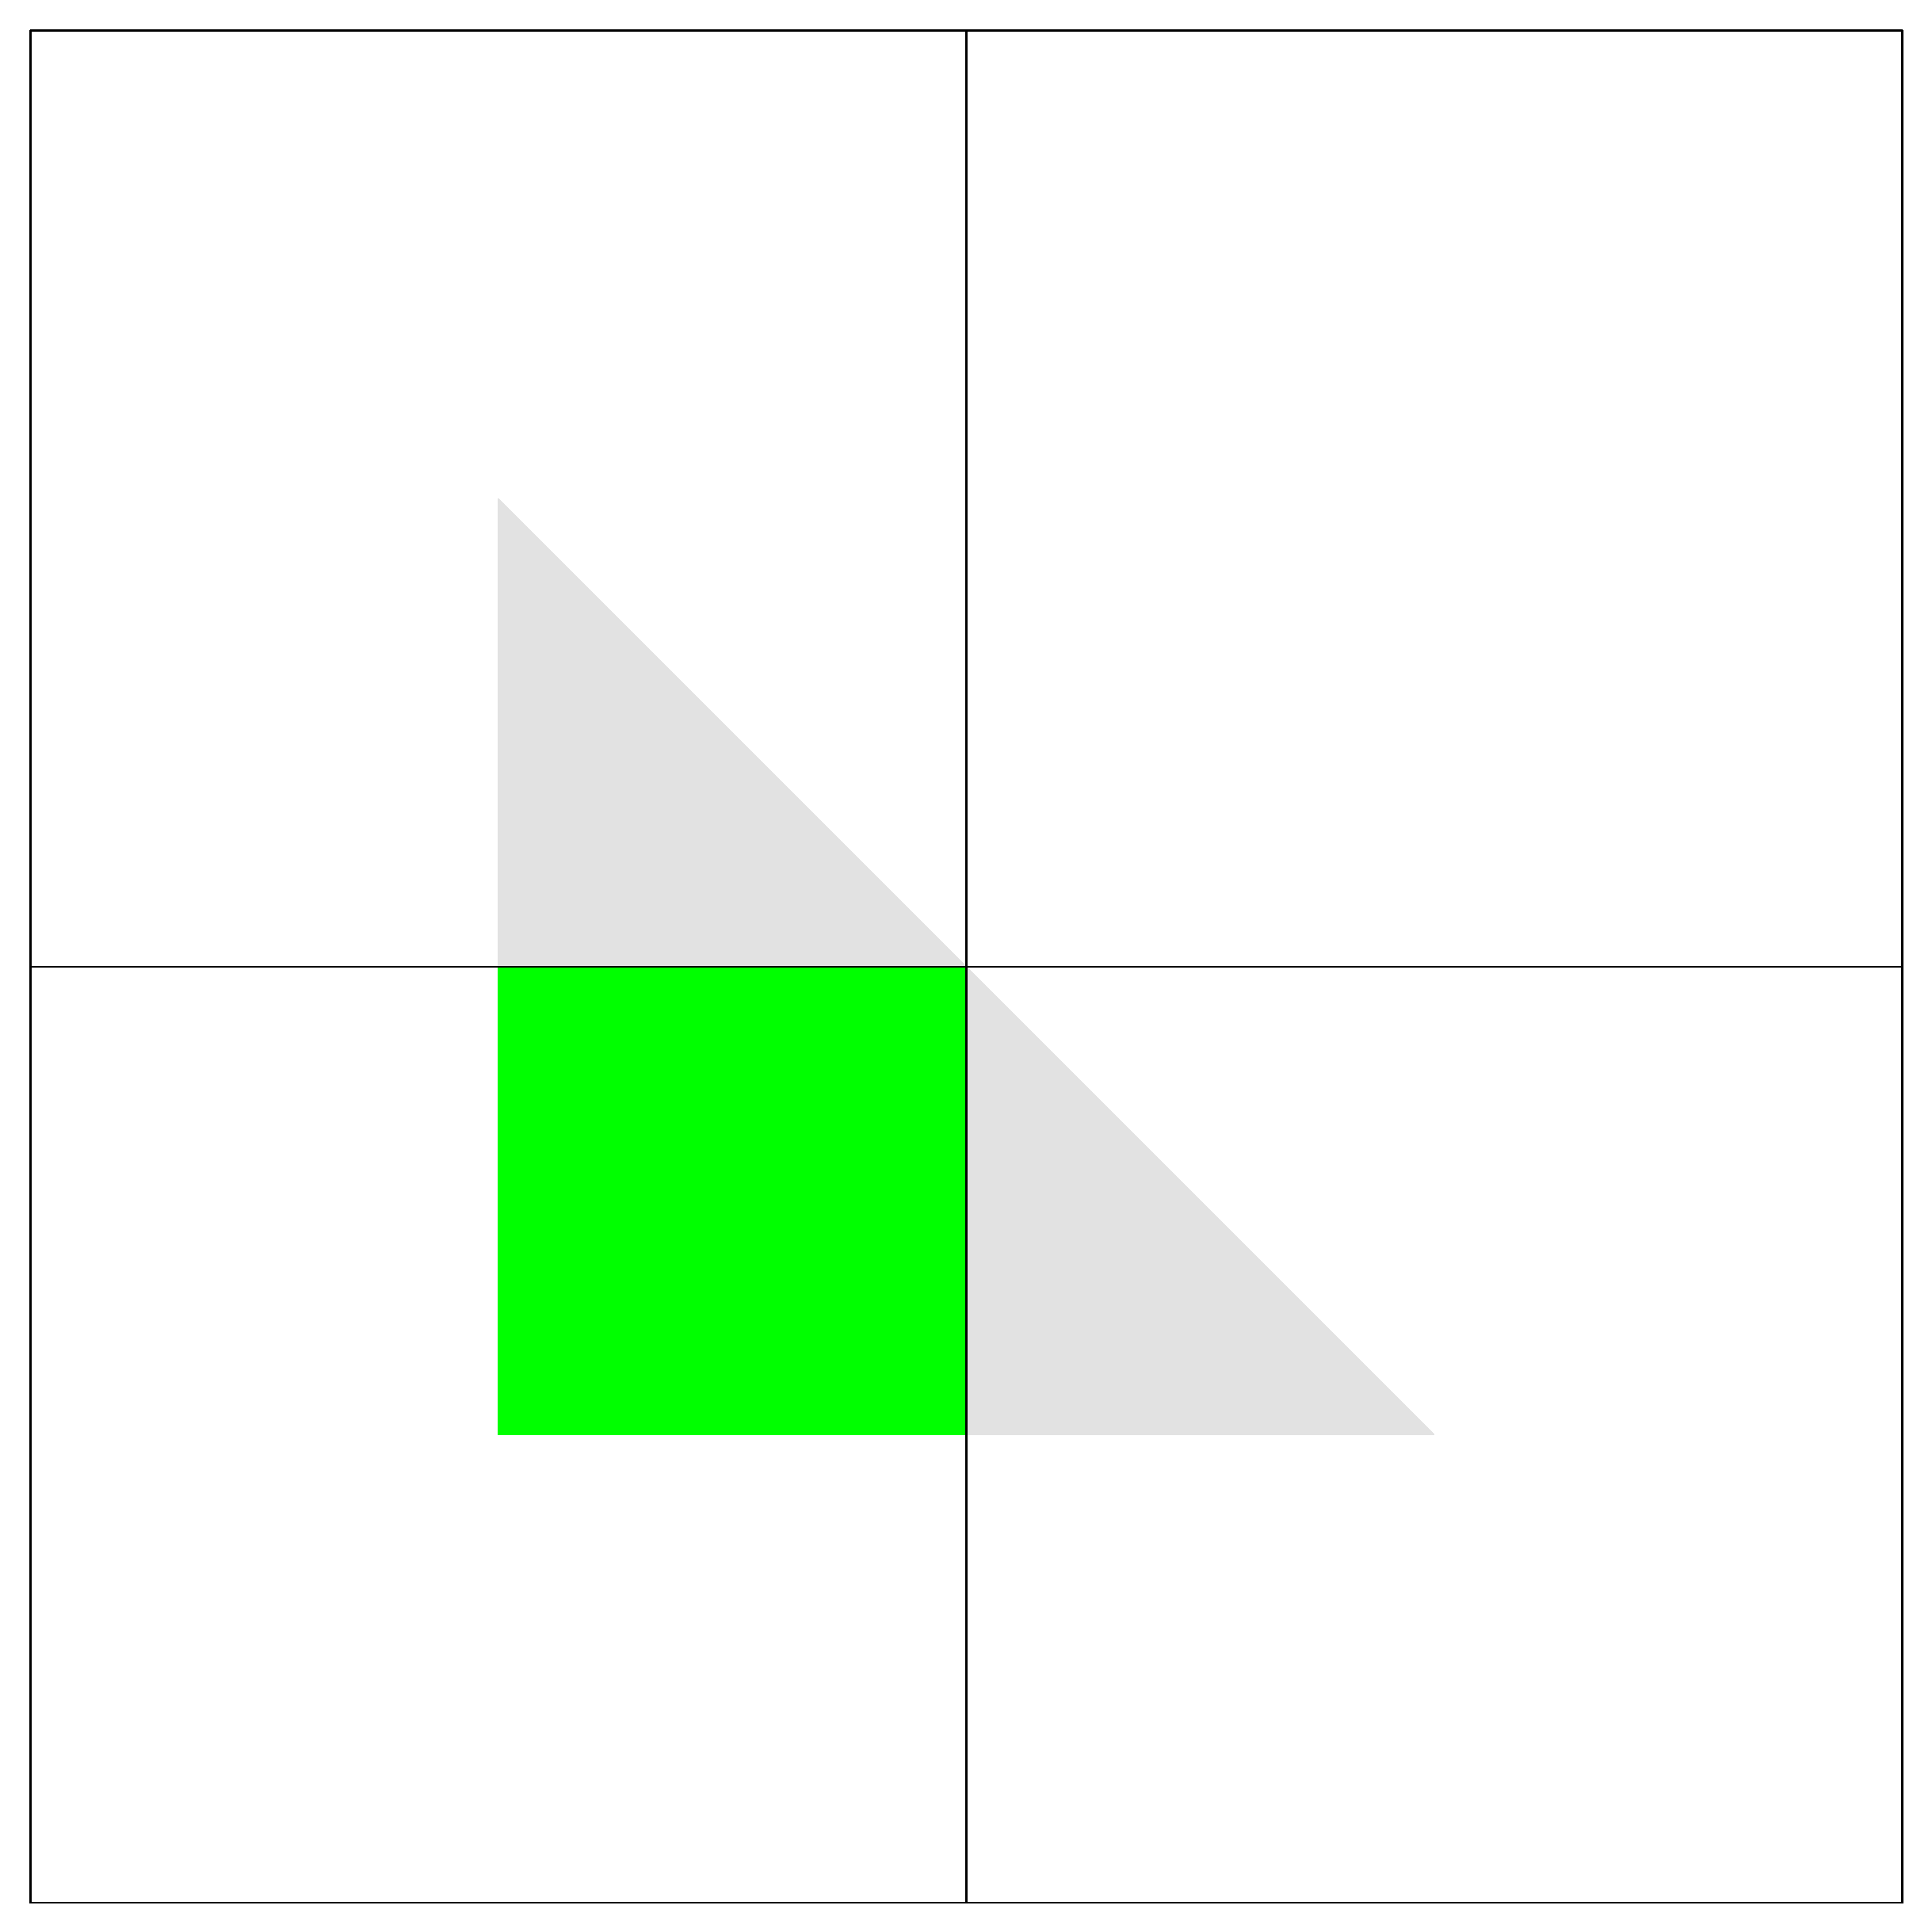
\includegraphics[width=\linewidth]{drawings/cubes_01.pdf}
  Voxel 1 
  
  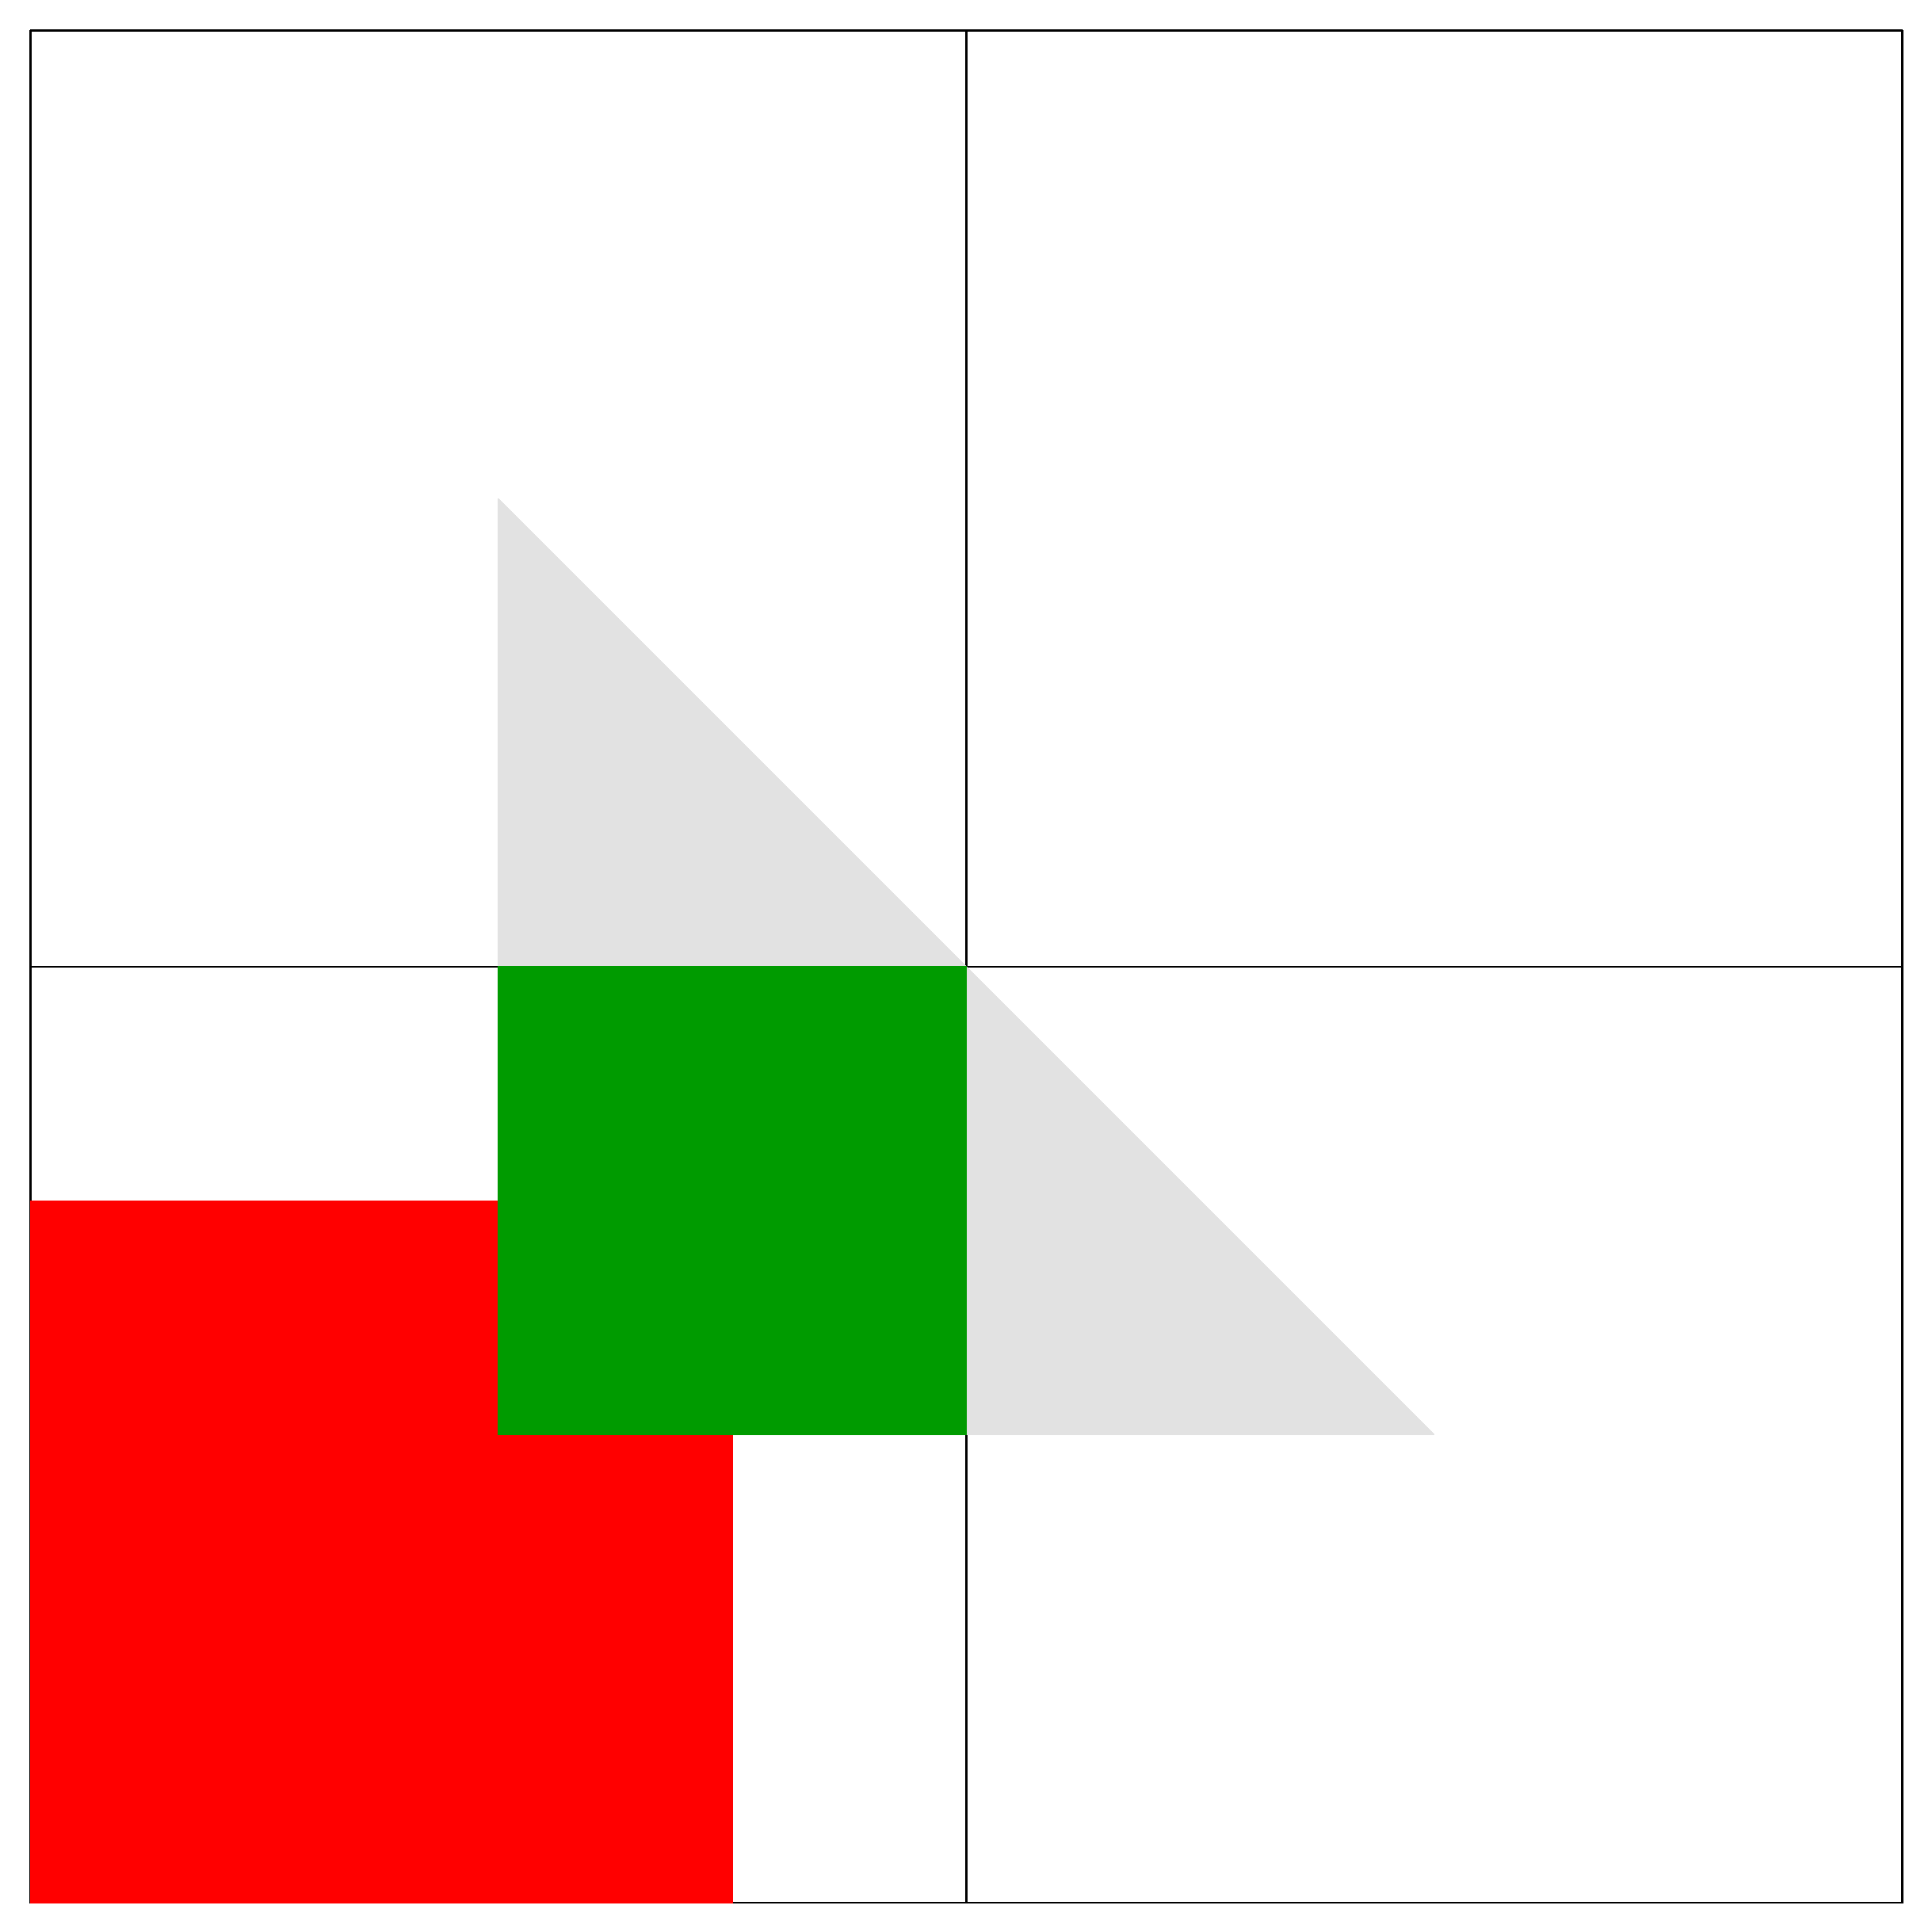
\includegraphics[width=\linewidth]{drawings/cubes_05.pdf}
  Voxel 5
\endminipage\hfill
\minipage{0.25\textwidth}
  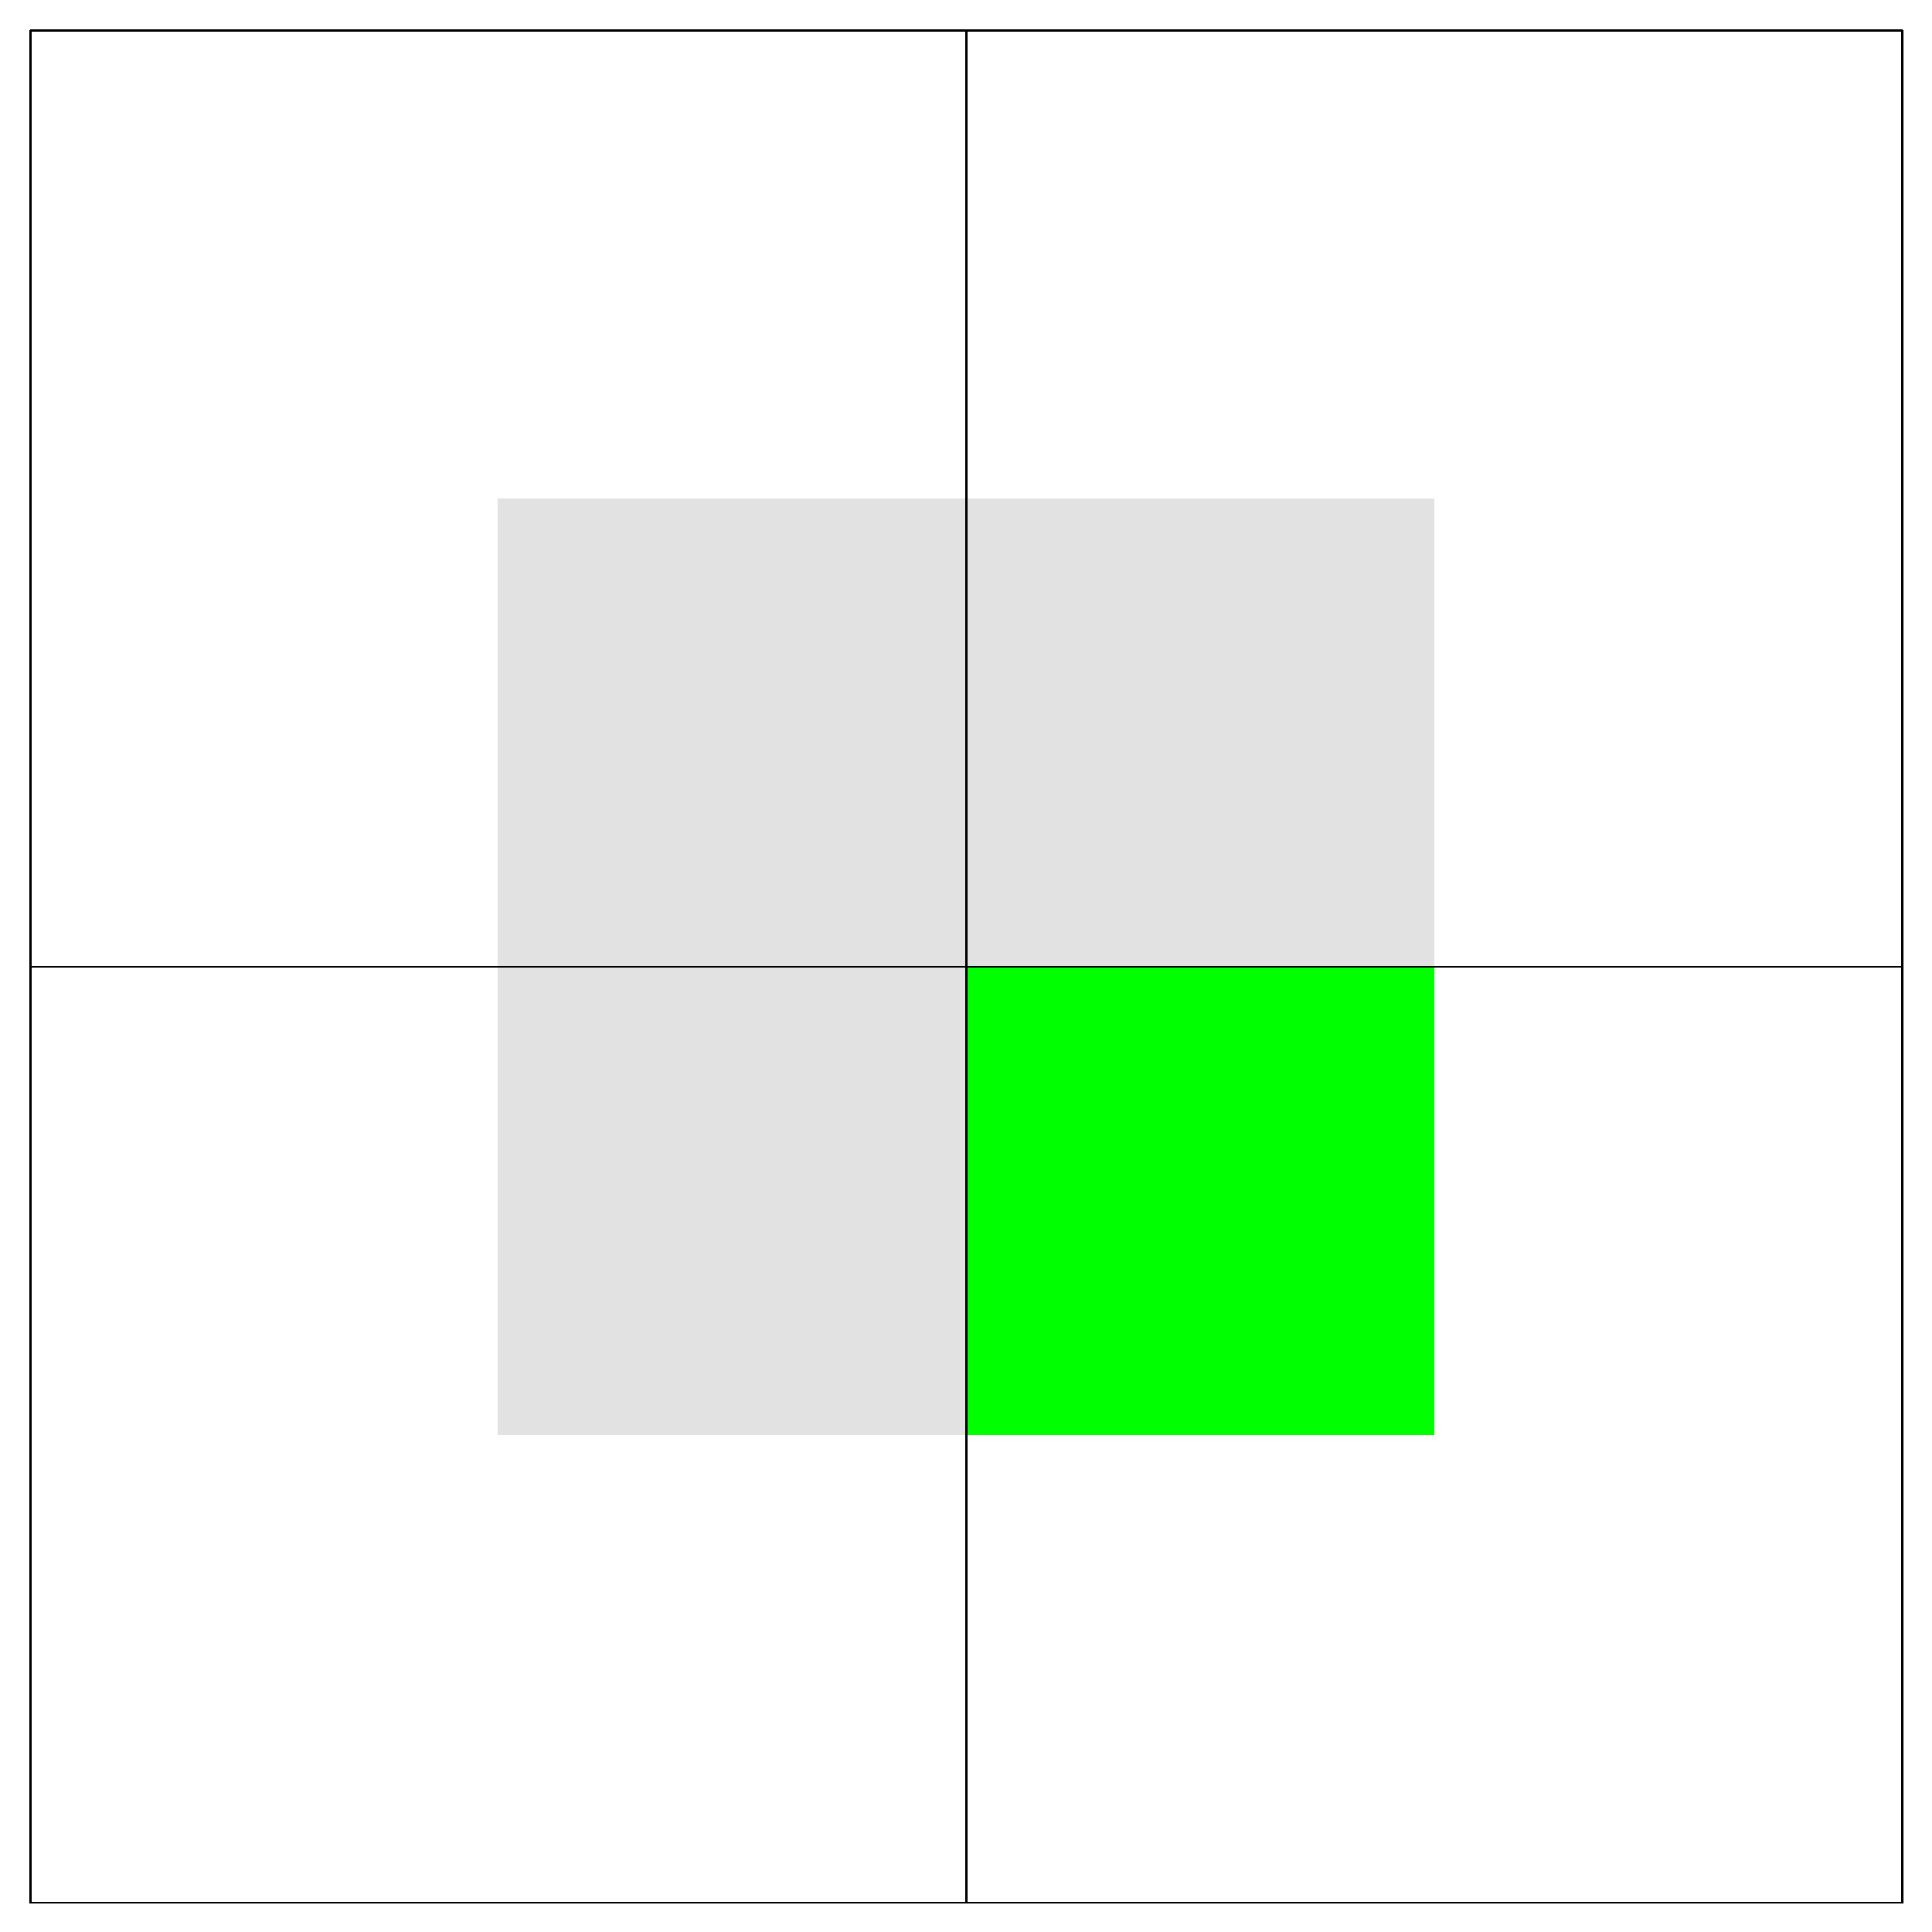
\includegraphics[width=\linewidth]{drawings/cubes_02.pdf}
  Voxel 2
  
  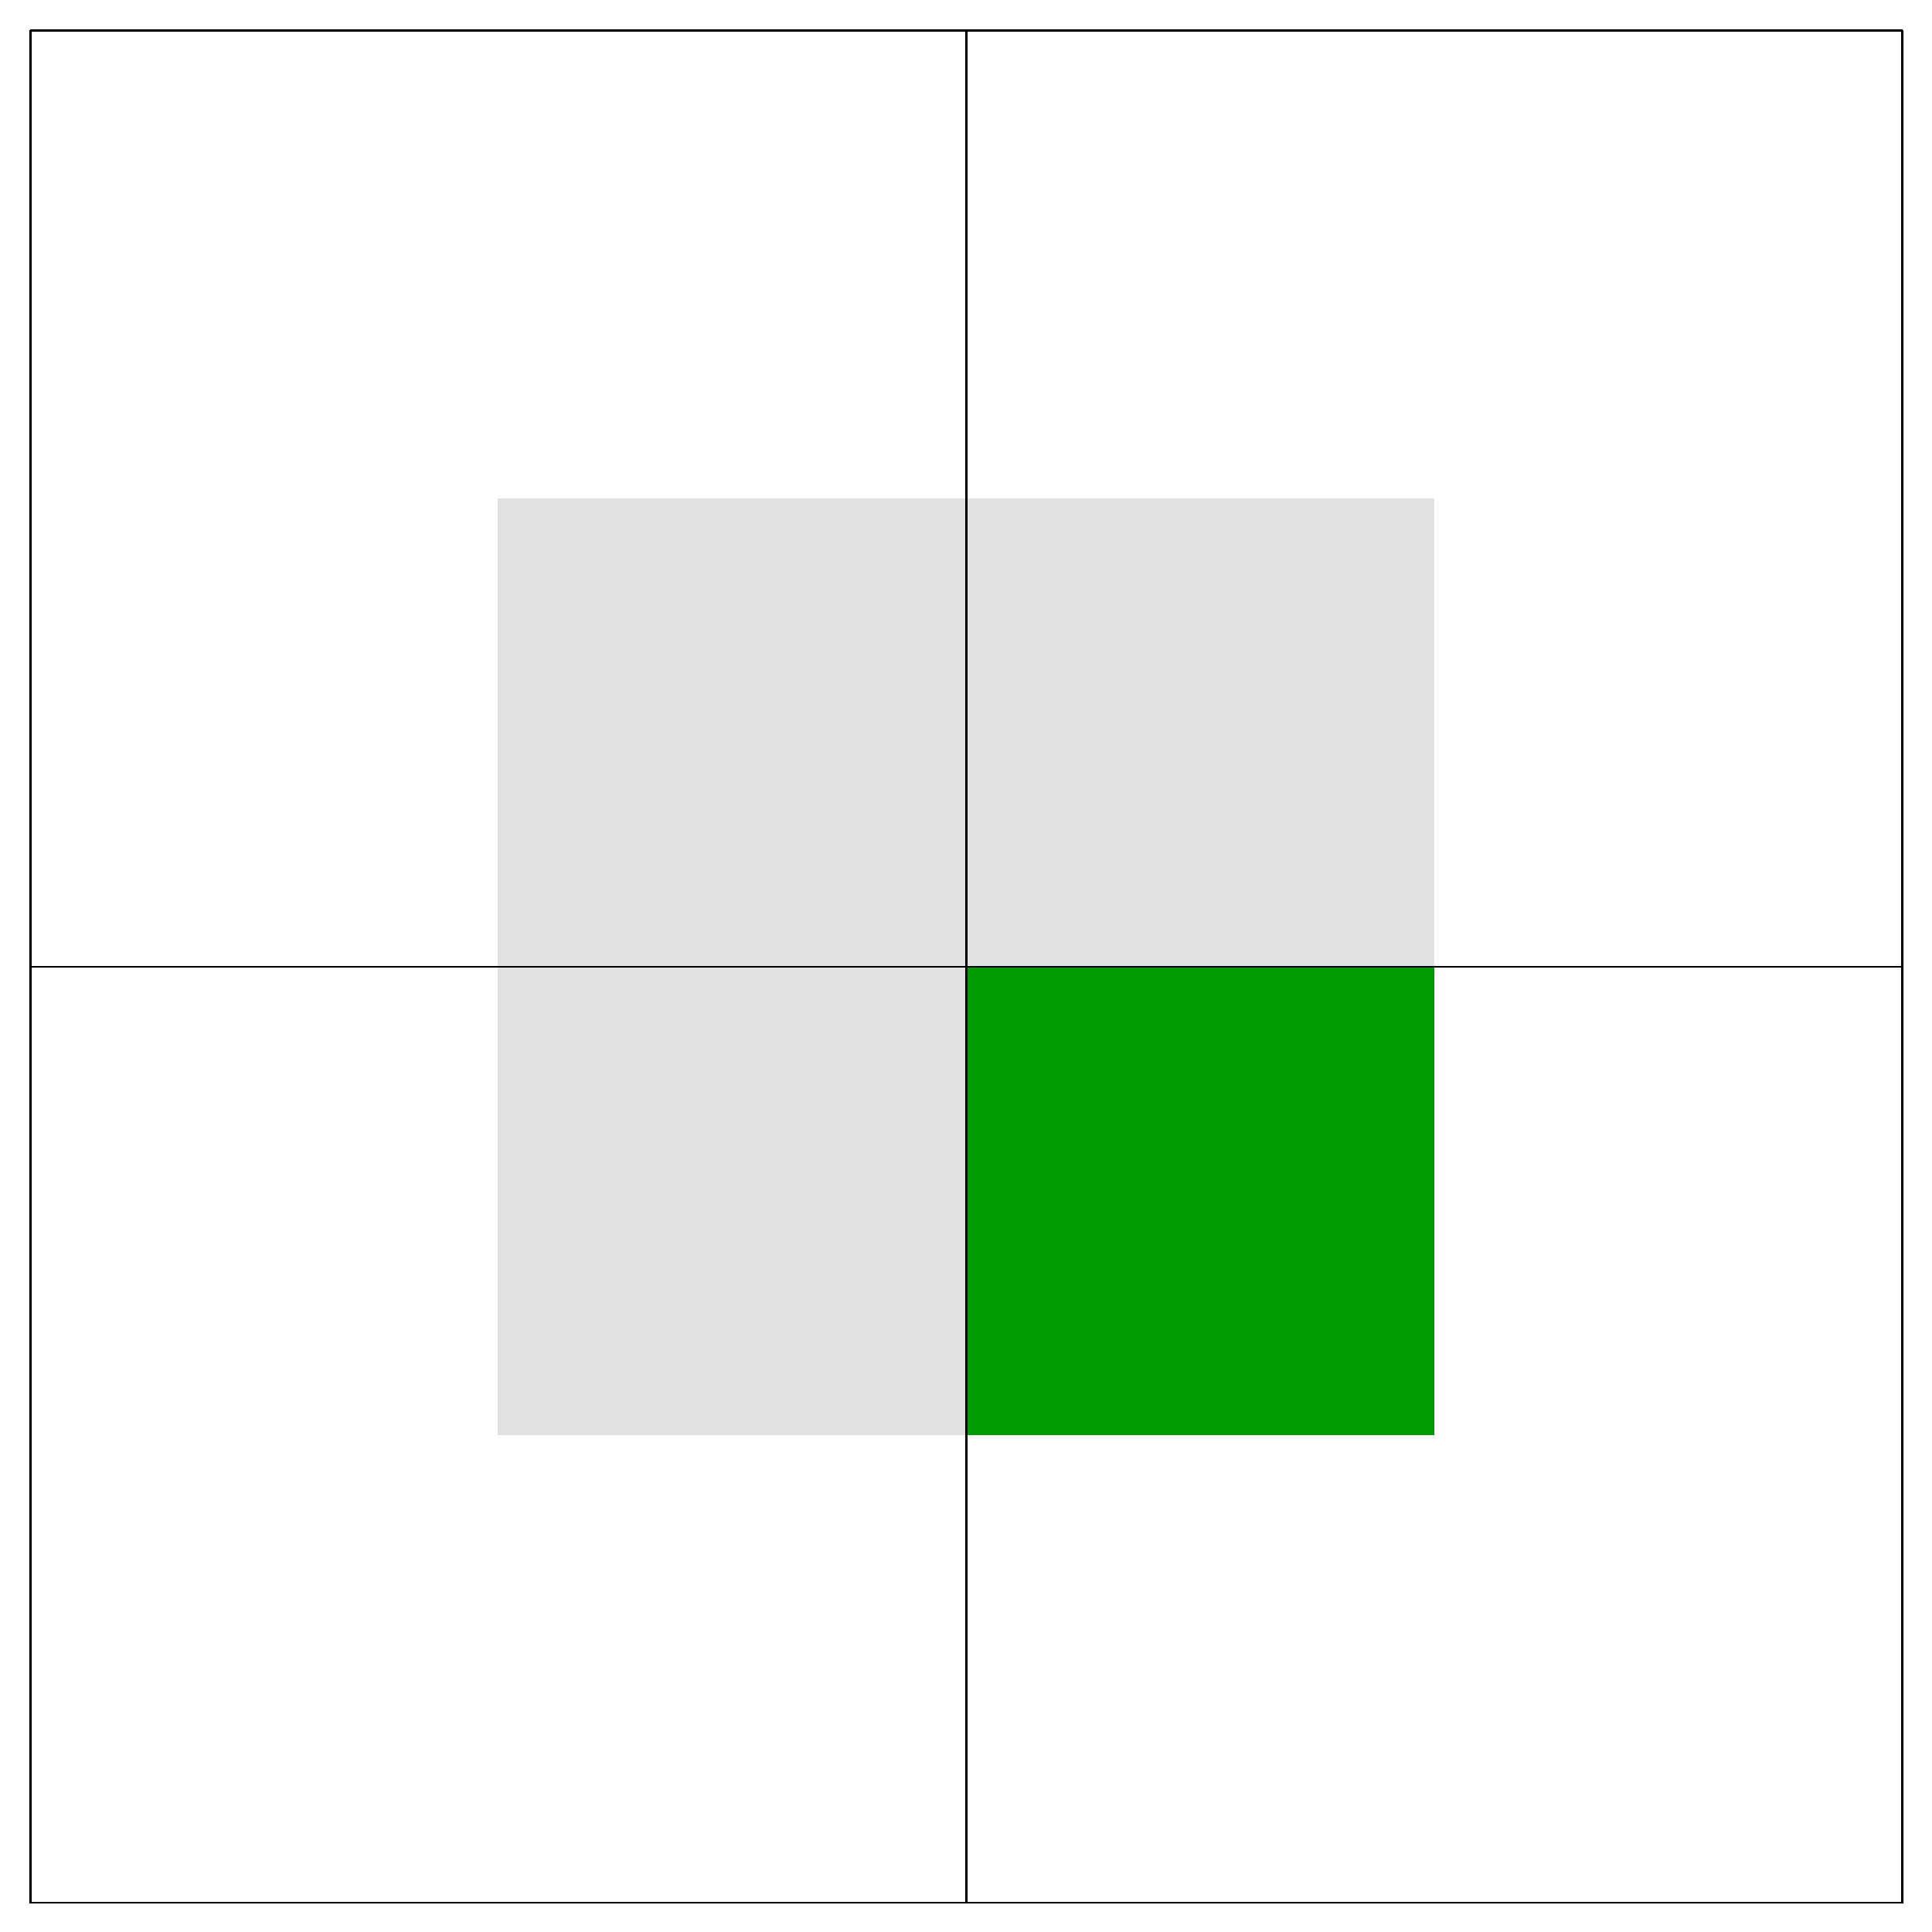
\includegraphics[width=\linewidth]{drawings/cubes_06.pdf}
  Voxel 6
\endminipage\hfill
\minipage{0.25\textwidth}%
  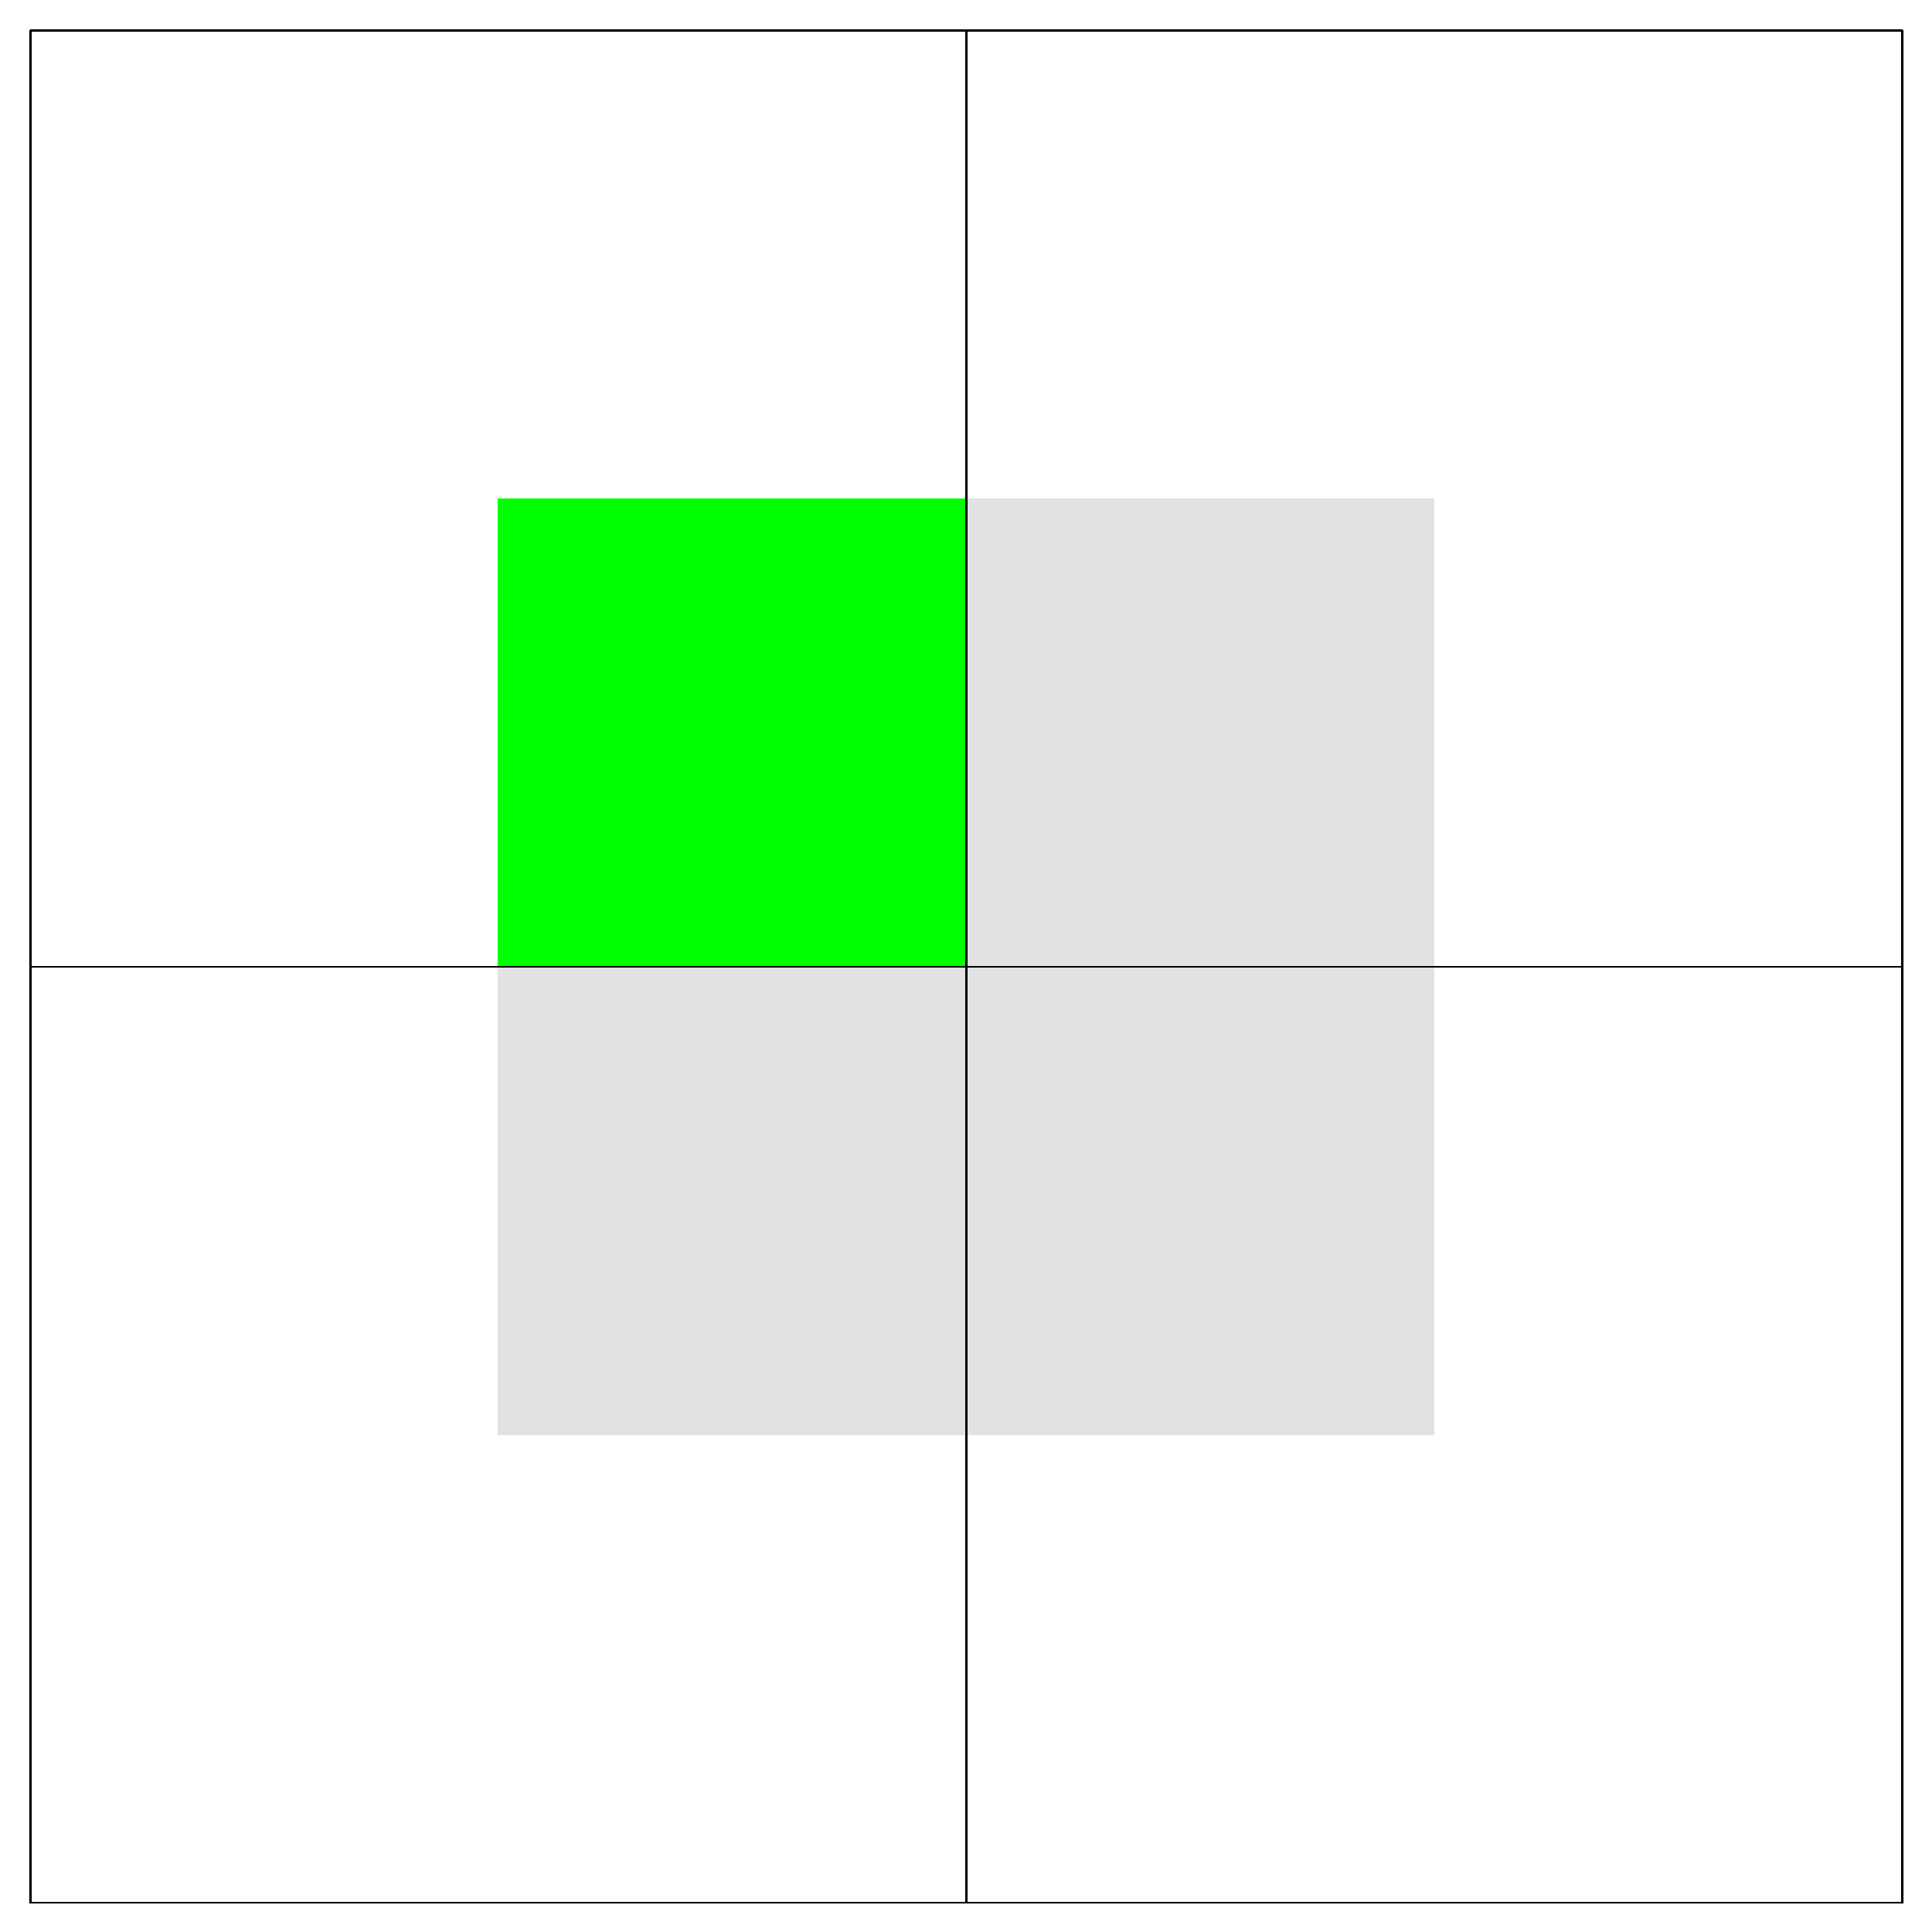
\includegraphics[width=\linewidth]{drawings/cubes_03.pdf}
  Voxel 3
  
  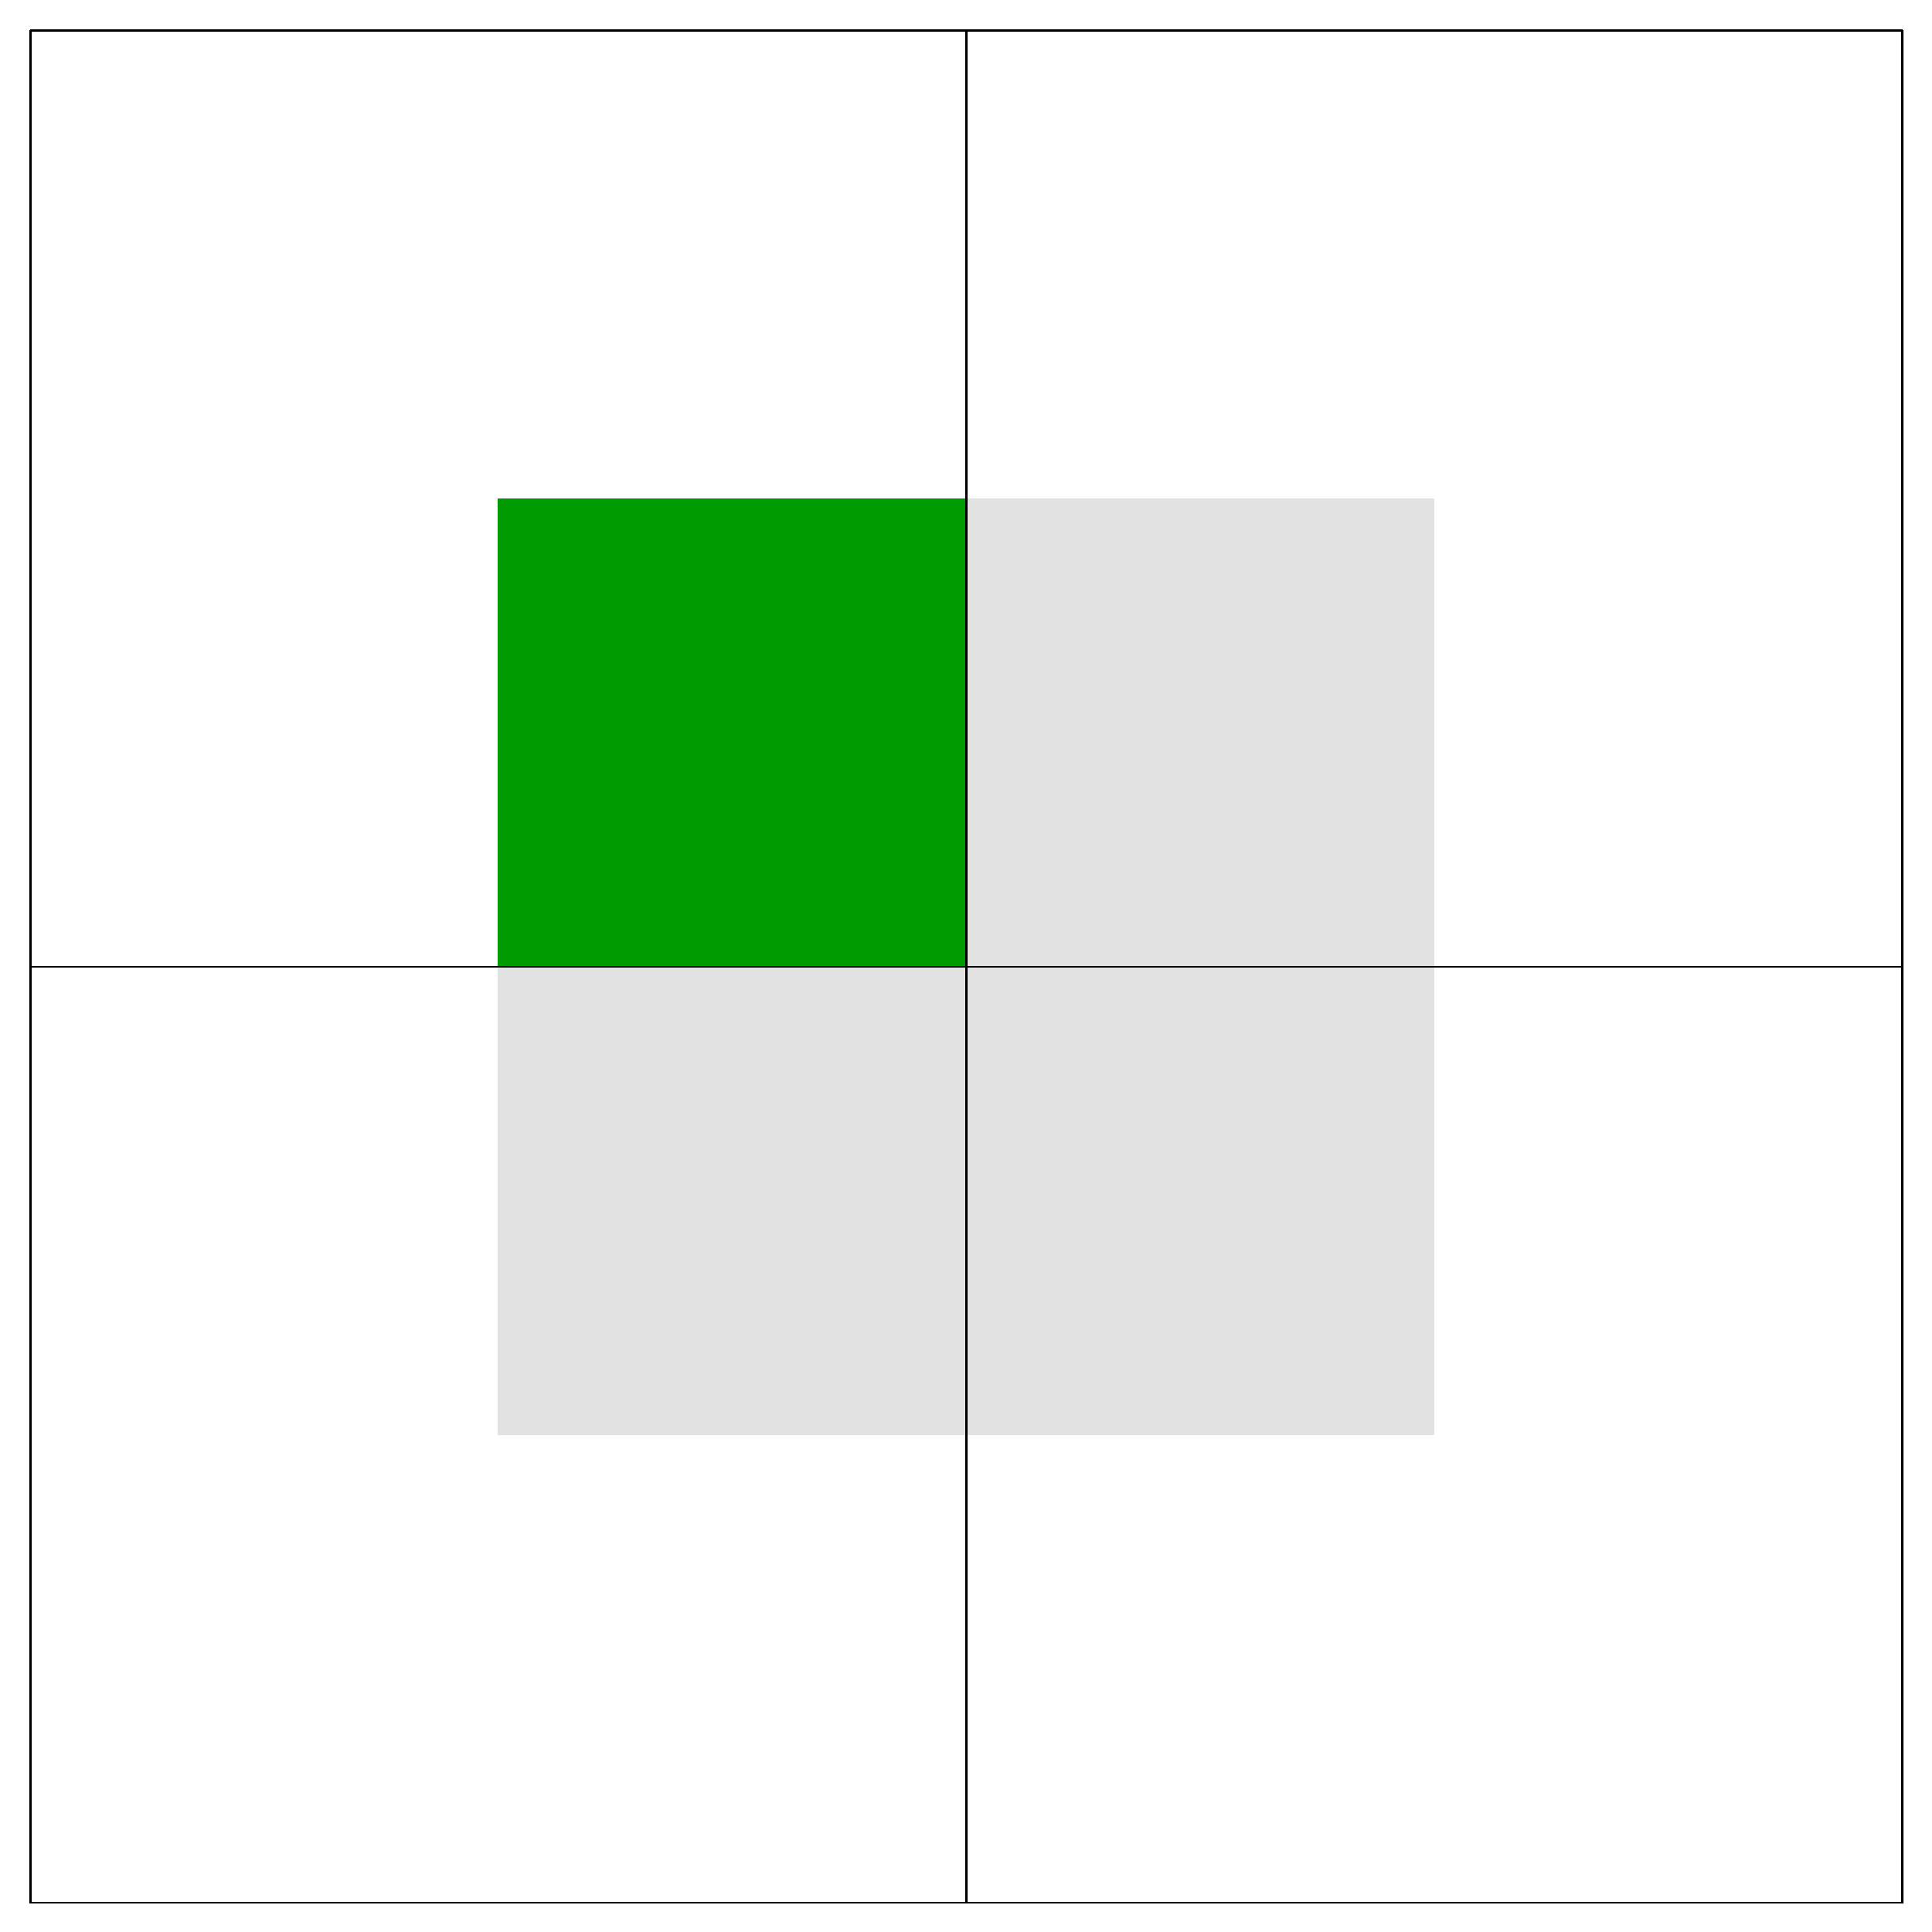
\includegraphics[width=\linewidth]{drawings/cubes_07.pdf}
  Voxel 7
\endminipage
\minipage{0.25\textwidth}%
  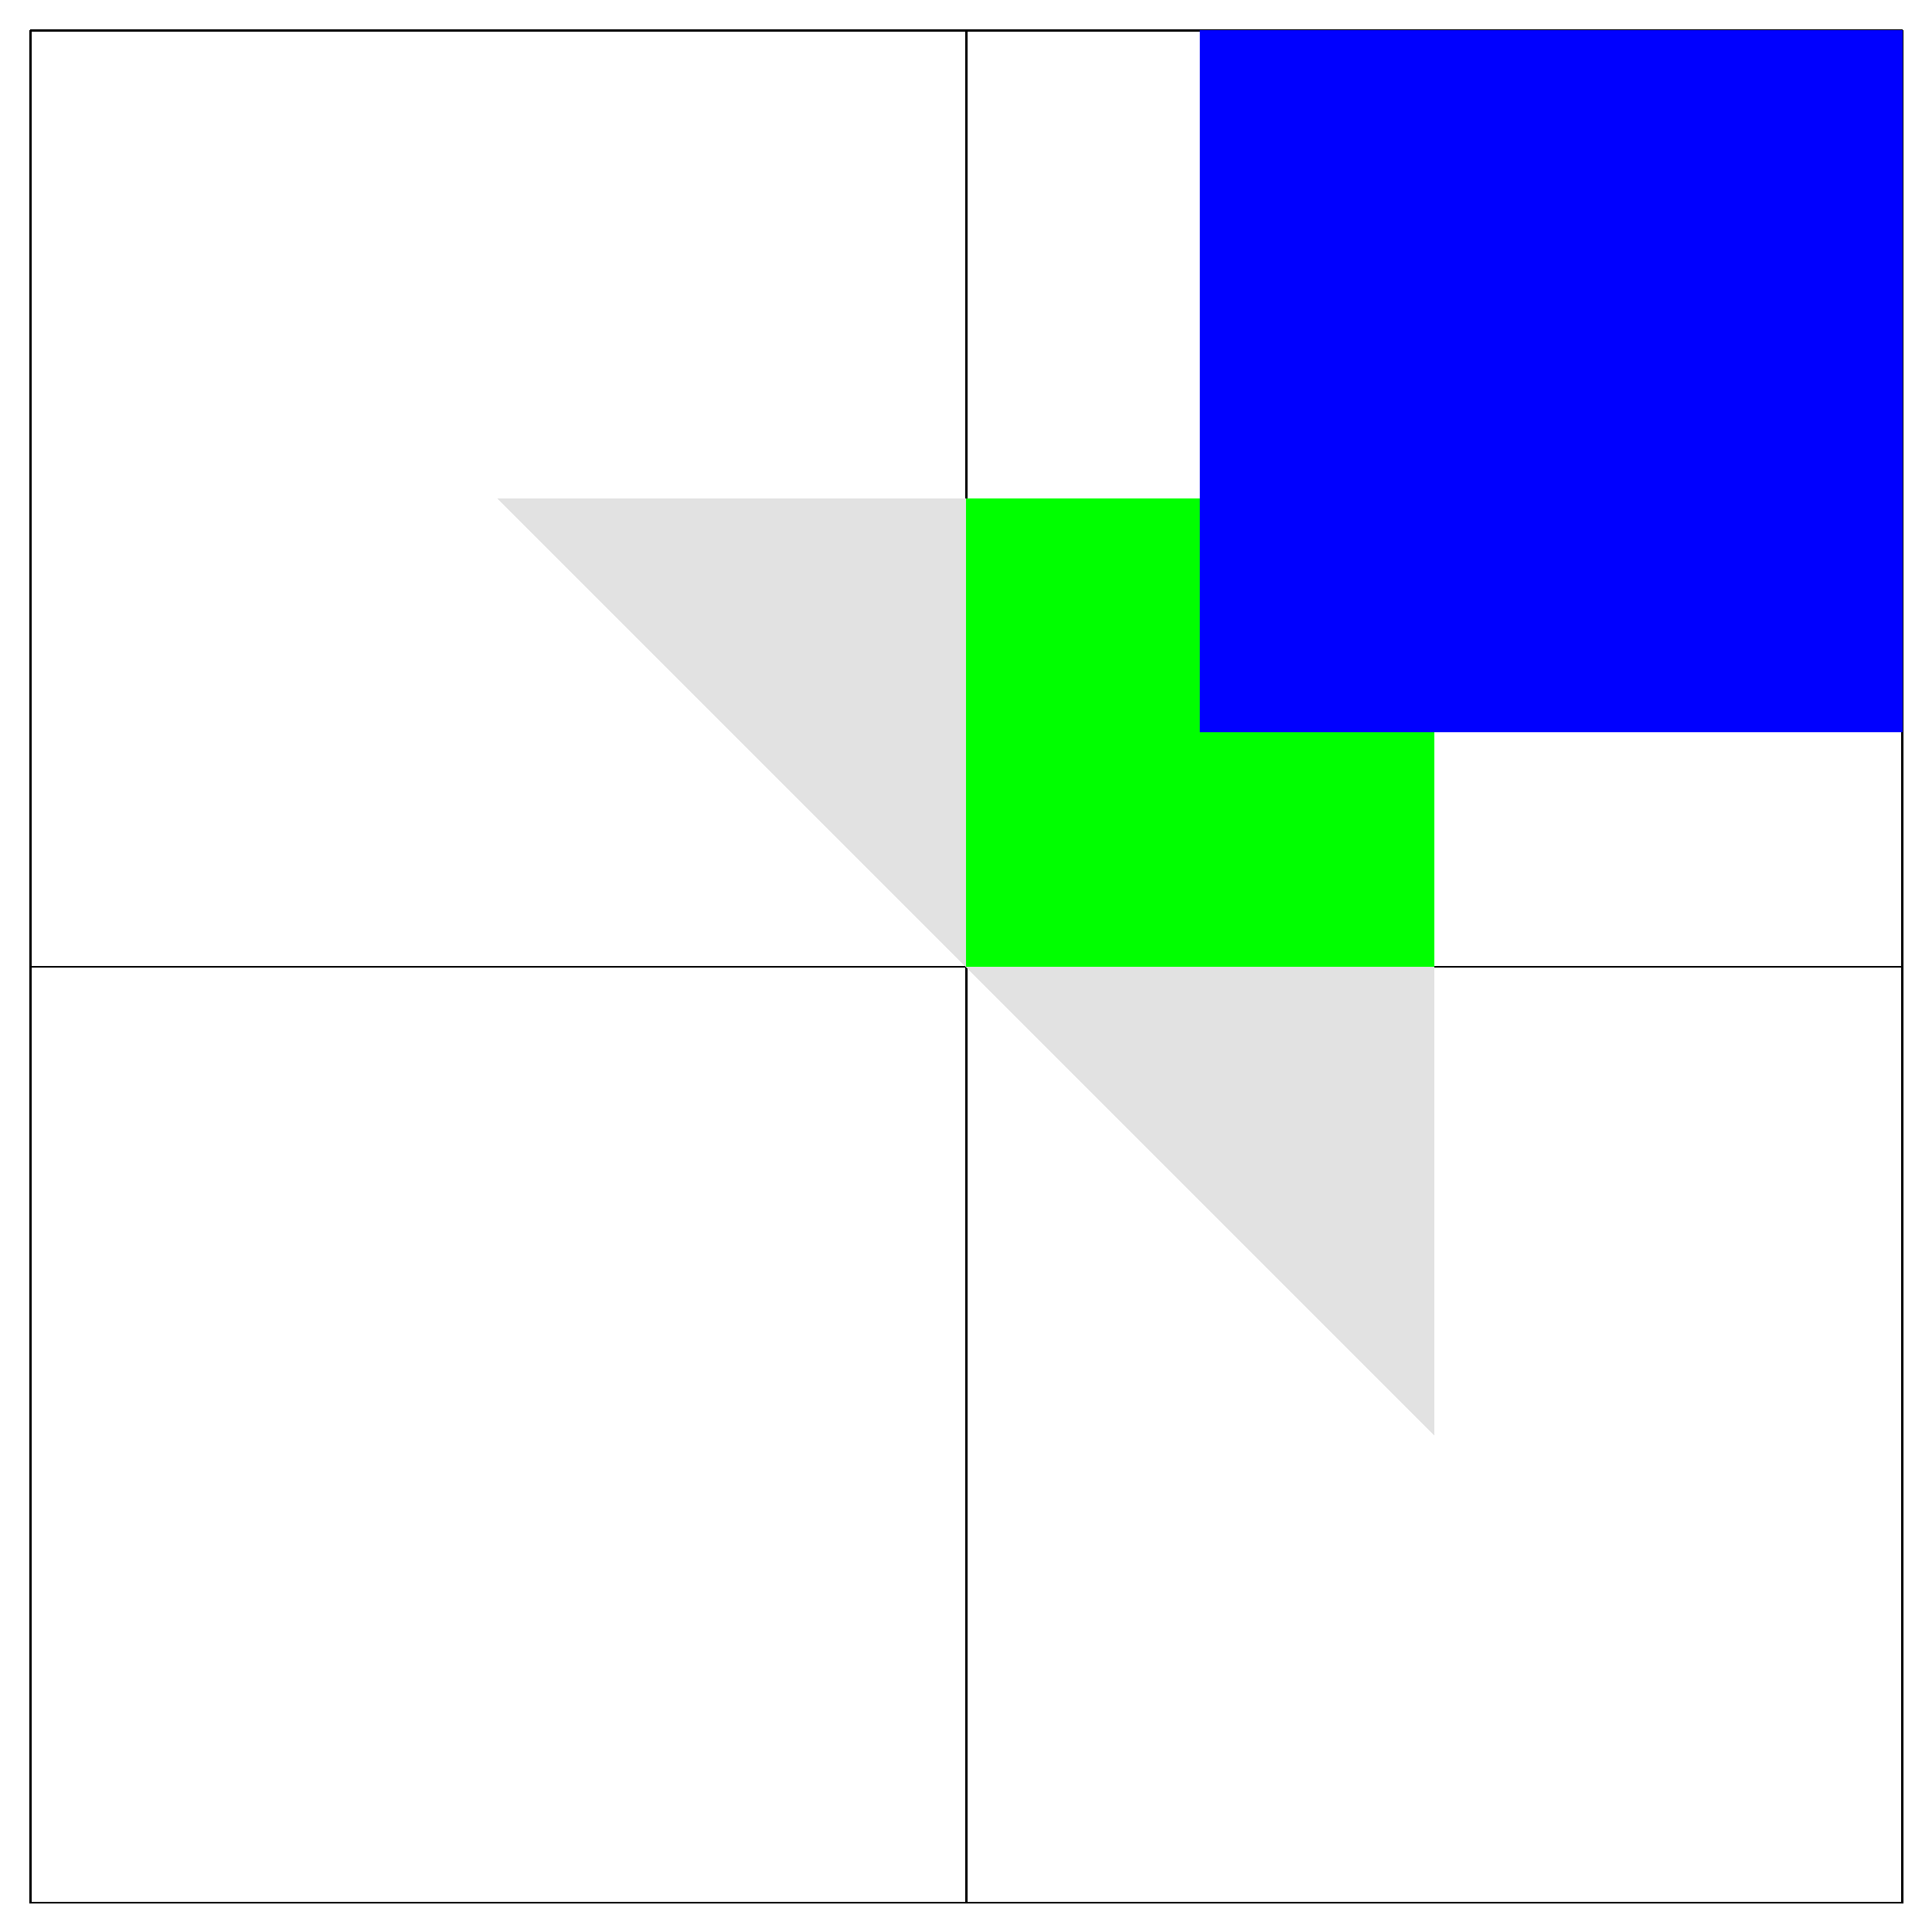
\includegraphics[width=\linewidth]{drawings/cubes_04.pdf}
  Voxel 4
  
  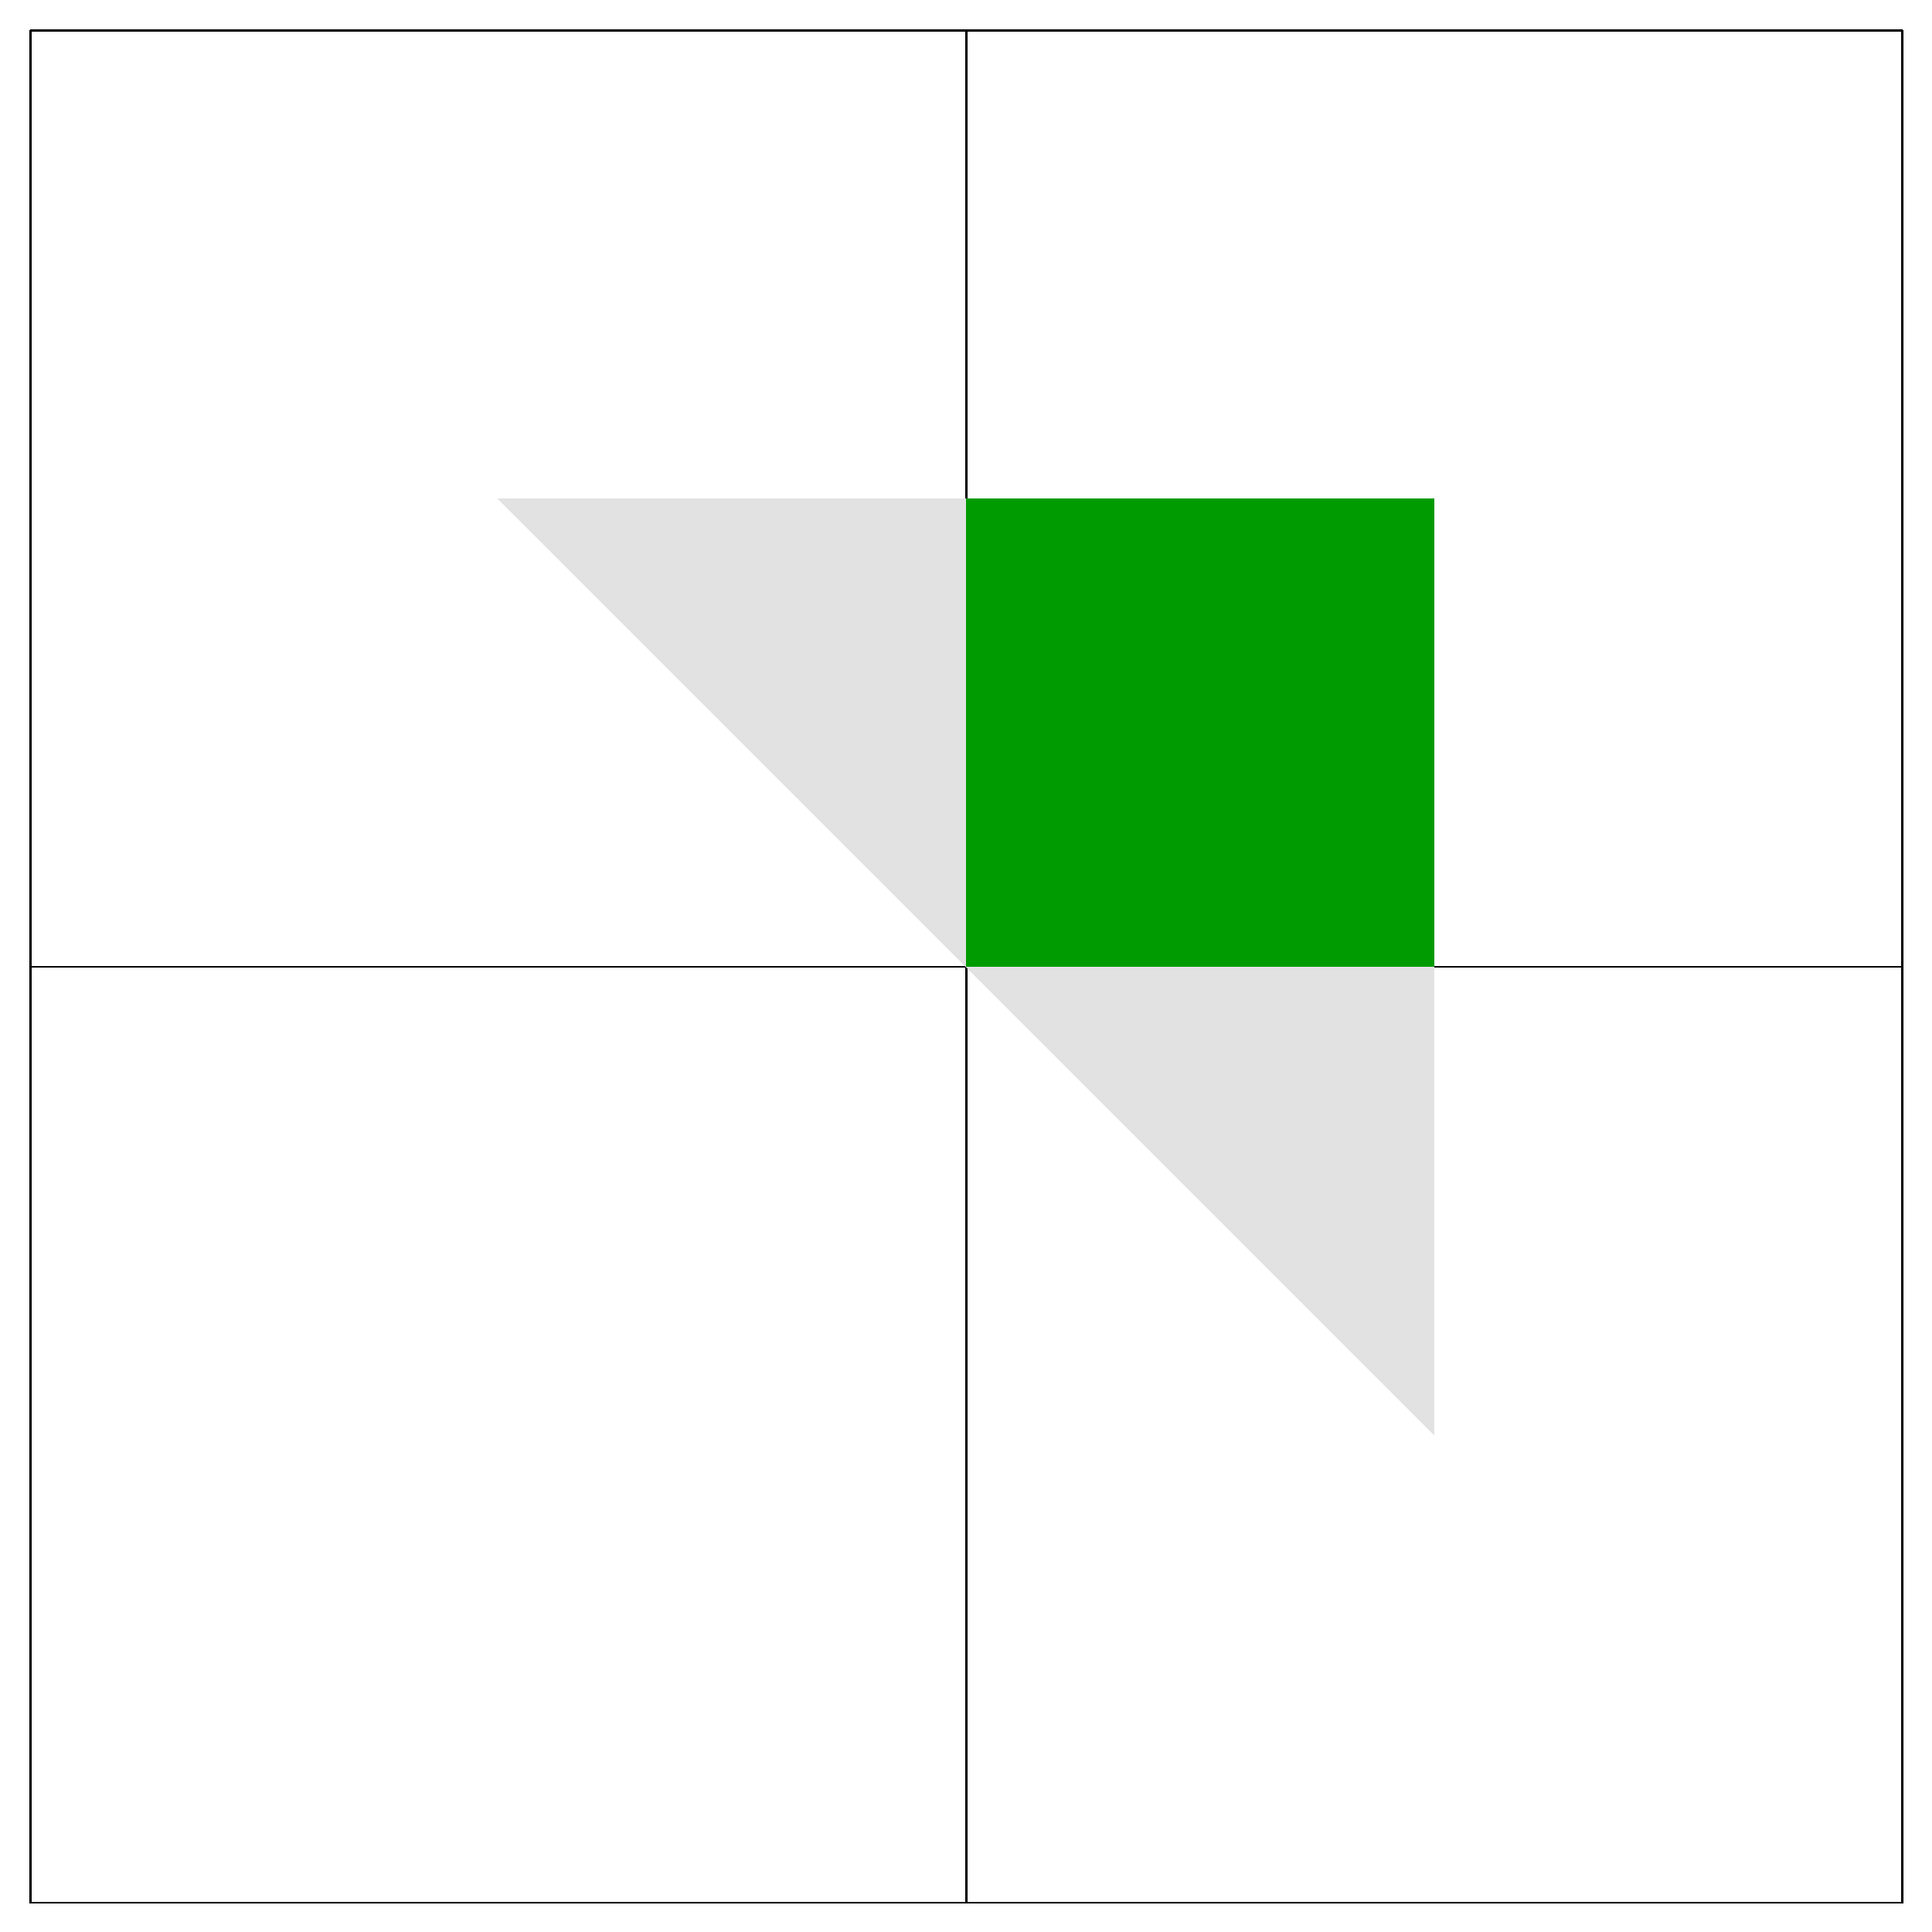
\includegraphics[width=\linewidth]{drawings/cubes_08.pdf}
  Voxel 8
\endminipage
\caption{Orthographic perspective of the images produced by each traced voxel}
\label{fig:cubes}
\end{figure}

\begin{figure}[!htb]
\centering
  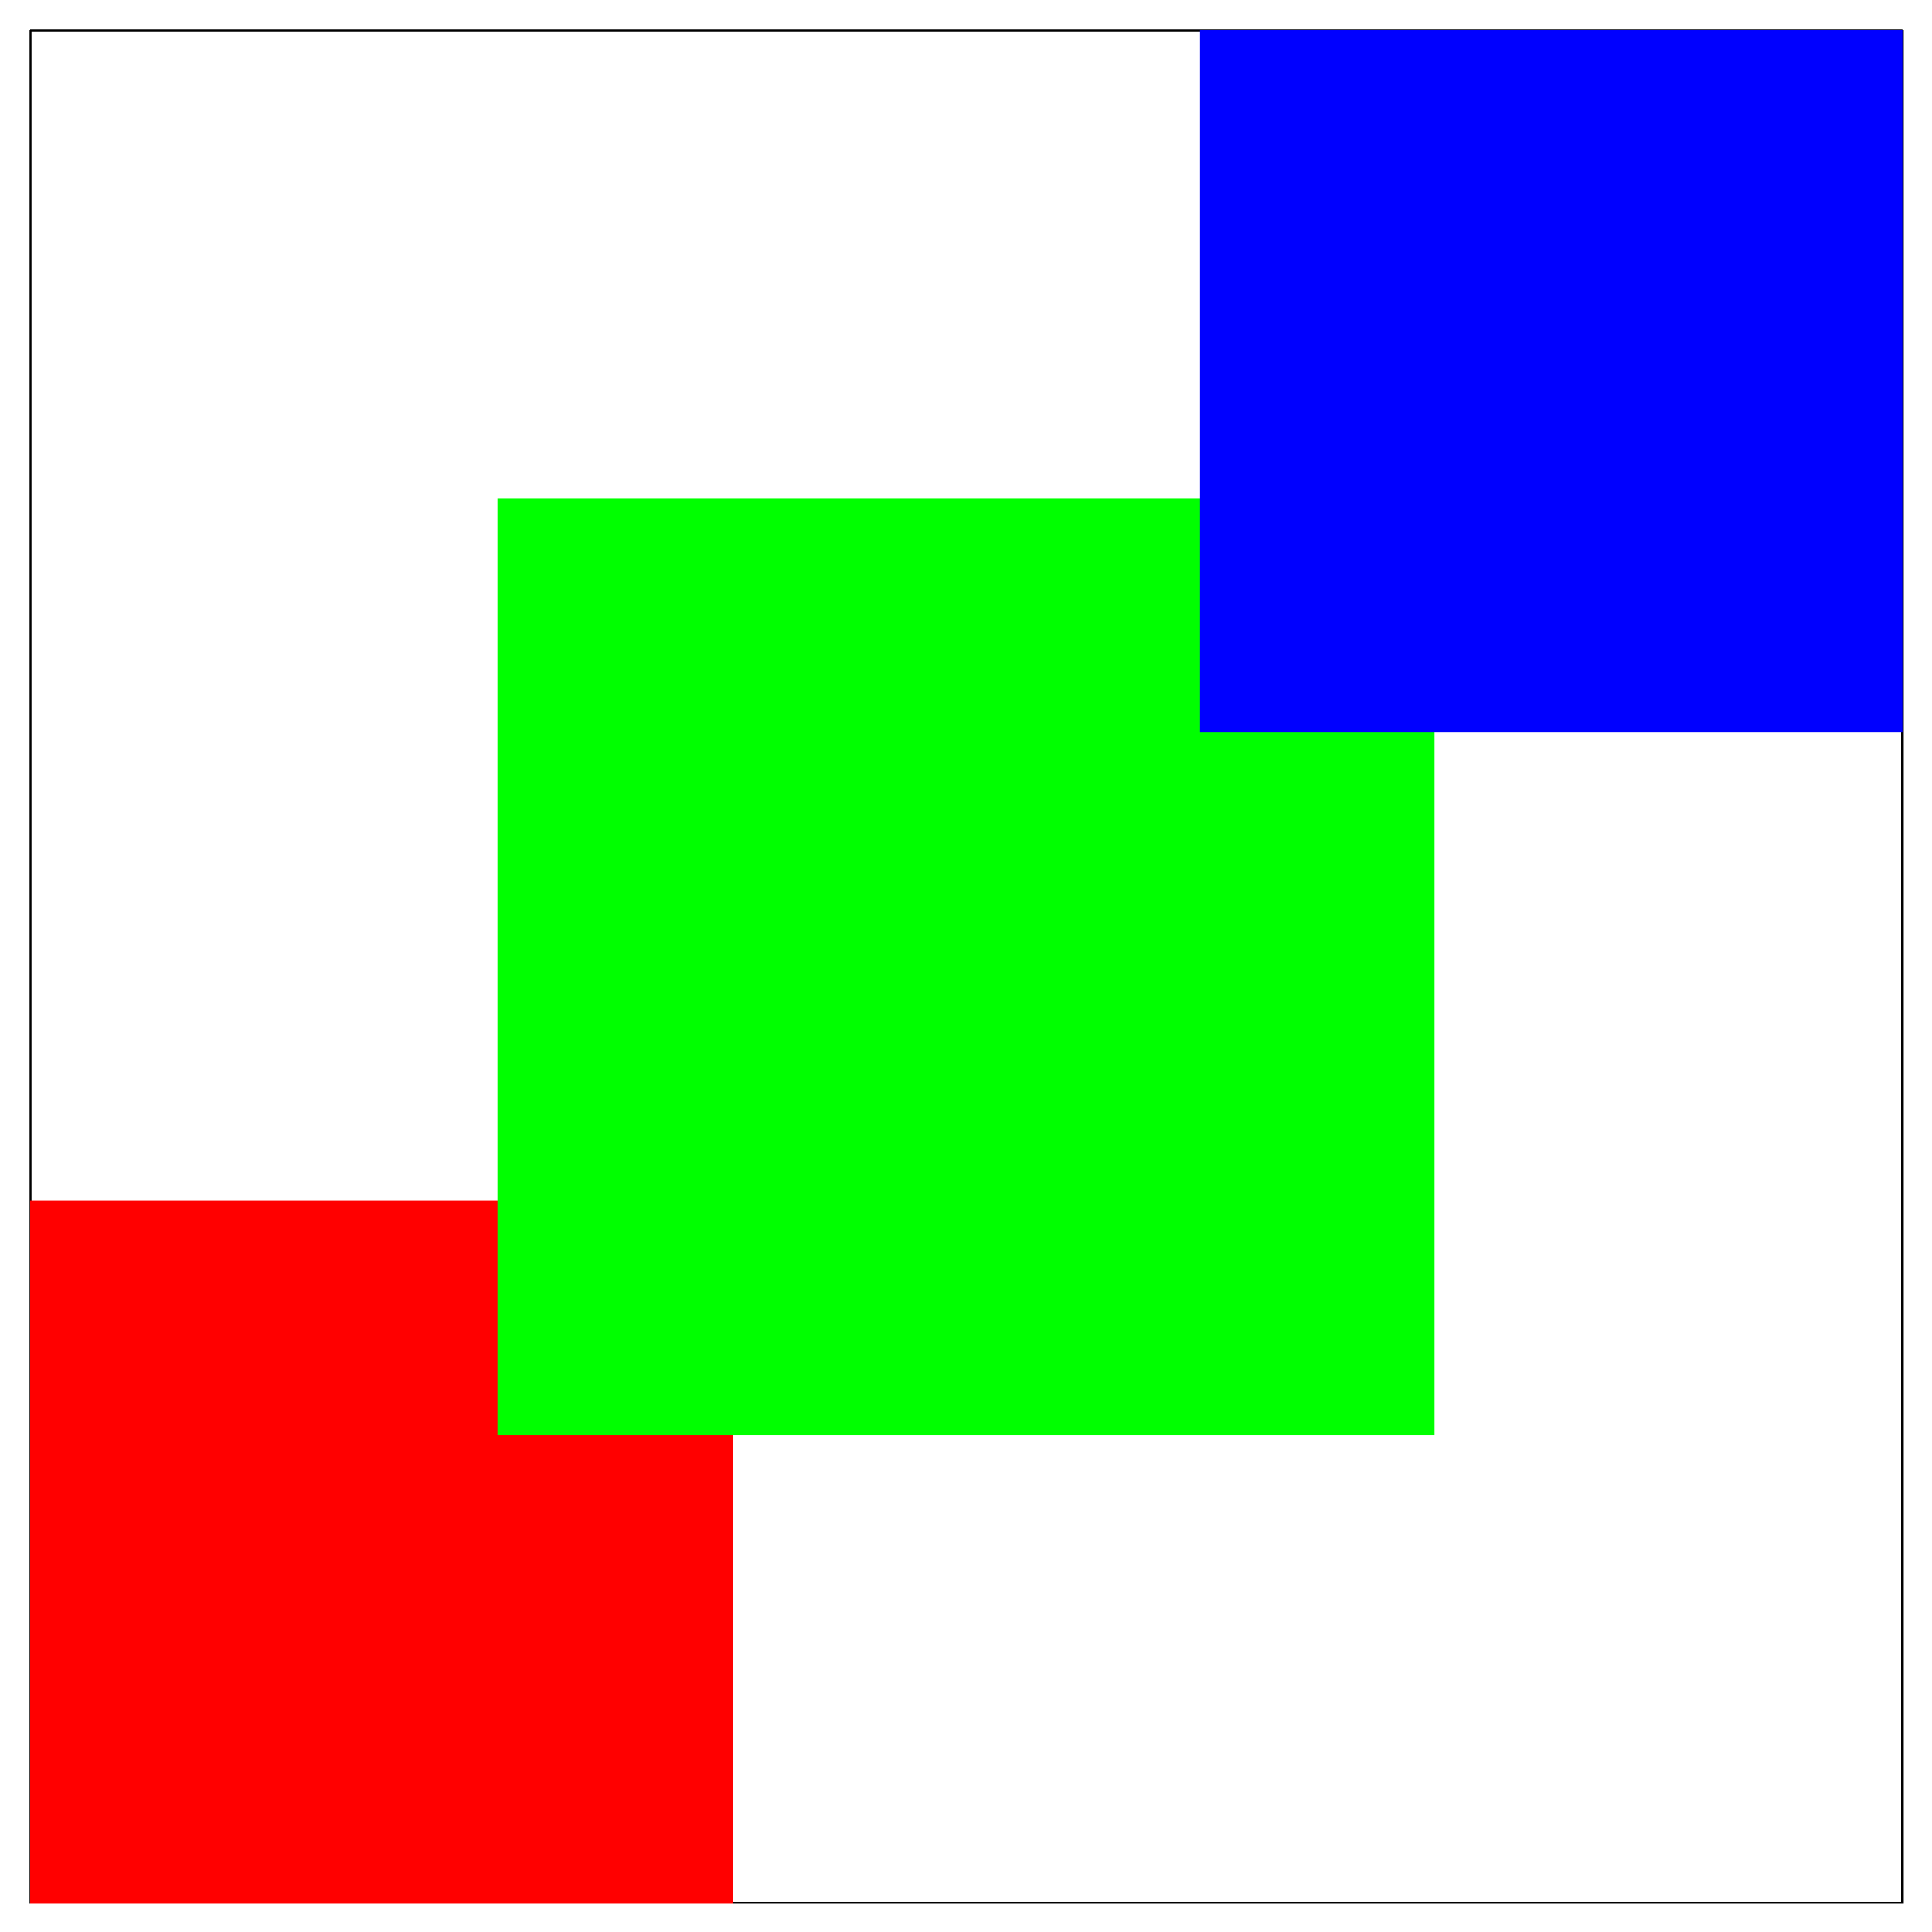
\includegraphics[height=5cm]{drawings/cube_final.pdf}
\caption{Orthographic perspective of the final composed image of traced voxels}
\label{fig:cubes_final}
\end{figure}


\subsection{Communication avoiding ray tracing}
\label{sec:ca-ray-tracing}

Expanding on the ray casting algorithm, we will now look at how we might design 
similar communication avoiding algorithms to implement a full ray tracer.  We 
will first tackle secondary shadow rays.  Shadow rays are rays cast from an 
intersection point that point in the direction of a light source.  To correctly 
compute shadows, it is important to know if the ray intersects with any other 
objects in the scene anywhere along its path from the intersection point of the 
object to the light source.  

Shadow ray calculations could result in a significant amount of communication if
done during runtime.  To reduce this cost, we introduce a technique that 
distributes light information to each voxel prior to runtime.  Similar to the 
ray casting algorithm, we can cast rays into the scene from each light source.  
Instead of sending all rays to all voxels however, we will need to propagate the
rays through the scene, starting with the light source and moving outward.  As
the rays are propagated they can be marked as in shadow or not.  As the light
rays reach a new voxel, they produce a mesh on the facing wall.  Each vertex in
the mesh then contains either an indicator that the vertex is in shadow or
the direction and illumination information from its light source, see 
figure~\ref{fig:light-distribution}.  Additional information on 
implementation can be found in section~\ref{sec:proposed_algorithm}.

\begin{figure}[!htb]
\centering
\begin{subfigure}{0.49\textwidth}
 \centering
  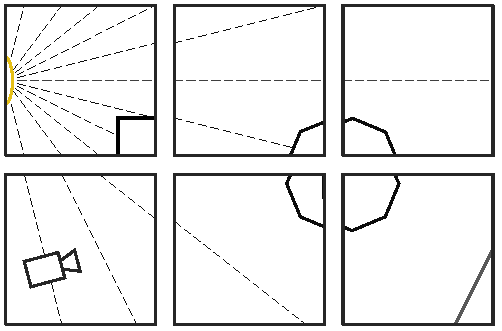
\includegraphics[width=.98\columnwidth]{drawings/Lights1.pdf}
  \caption{Initial light rays}
\end{subfigure}
\begin{subfigure}{0.49\textwidth}
 \centering
  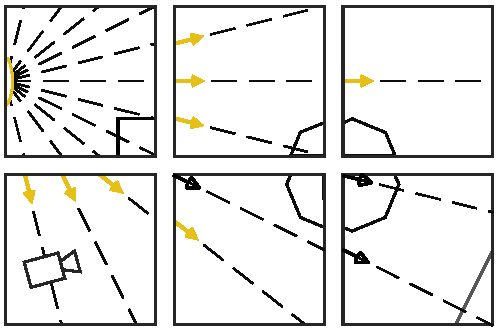
\includegraphics[width=.98\columnwidth]{drawings/Lights2.pdf}
  \caption{Computed light mesh}
\end{subfigure}
\caption{Light ray distribution}
\label{fig:light-distribution}
\end{figure}

The computed light is then used at runtime by the voxel computation to 
compute secondary shadow rays without needing to communicate with any other 
voxel.  The individual voxel, using the location of each light source can 
compute rays from an intersection point to each light source.  At the 
intersection of the ray with a voxel wall, the corresponding light mesh will be 
used to determine the correct illumination necessary for the intersection point.
A nearest neighbor or averaging algorithm can be used to determine which vertex 
or vertices in the mesh are closest to the intersection point.  This information
can be used to interpolate and illuminate the intersection point.

\subsubsection{Reflected and refracted rays}
Although not implemented within the scope of this thesis, we introduce a 
potential communication avoiding strategy for handling reflected and refracted 
rays.  For refracted rays, a technique similar to the light meshes could be 
used, where a mesh is computed from each reflected material and distributed 
outward to each voxel.  Instead of holding light and shadow information the 
vertices of the mesh would contain material information from the first object 
intersected.  Each voxel computation would then use the material mesh to 
determine the correct color for a reflected ray.  Each voxel would need access 
to all the material meshes in the case where a reflected ray reflects to another
reflector.  See section~\ref{sec:future-work} for additional details.

Refractor materials which change the trajectory of the rays that pass through 
them could be supported by the proposed algorithm through the use of a restart 
capability.  The underlying assumptions to compute the light and material meshes
rely on the rays maintaining a straight trajectory.  The same assumption is made
to compute the intersection of the viewing rays and each voxel they intersect 
with.  If a ray refracts in one voxel, the subsequent voxels would need to know 
the new intersection point of that ray and their wall, along with the rays new 
direction.  If we could detect when rays refract within a voxel and invalidate 
the computations being done with non-refracted rays, we could restart them with 
the correct rays.  Details on this technique can be found in 
section~\ref{sec:future-work}.

If a scene contains little or no reflected rays, the overhead of computing the
material meshes may outweigh the cost of communicating reflected rays at 
runtime.  If the material meshes and the light meshes are used however 
communication cost would be reduced to one pass through the domain for each 
light and each reflector prior to runtime.  At runtime each voxel's computation
would be an independent calculation, requiring no communication except to send
back the final results of the traced rays.  The use of meshes however, results 
in an approximation of the result produced by a conventional ray tracer due to 
the nearest neighbor or averaging used when a ray intersects the mesh.

\section{Proposed Algorithm}
\label{sec:proposed-algorithm}
Using a spatially even data distribution algorithm as described in 
section~\ref{sec:data_decomposition} and reducing communication as described in 
section~\ref{sec:communication} allows us to design the communication 
avoiding ray tracer outlined in figure~\ref{fig:design}.  The figure shows a 
Petri Net, see Section~\ref{sec:petri-nets}, describing the main components of 
a full ray tracing algorithm.  The following sections break down each place and
transition.  For the scope of this thesis we have implemented the highlighted 
section, details can be found in chapter ~\ref{sec:implementation}.

\begin{figure}[!htb]
\centering
  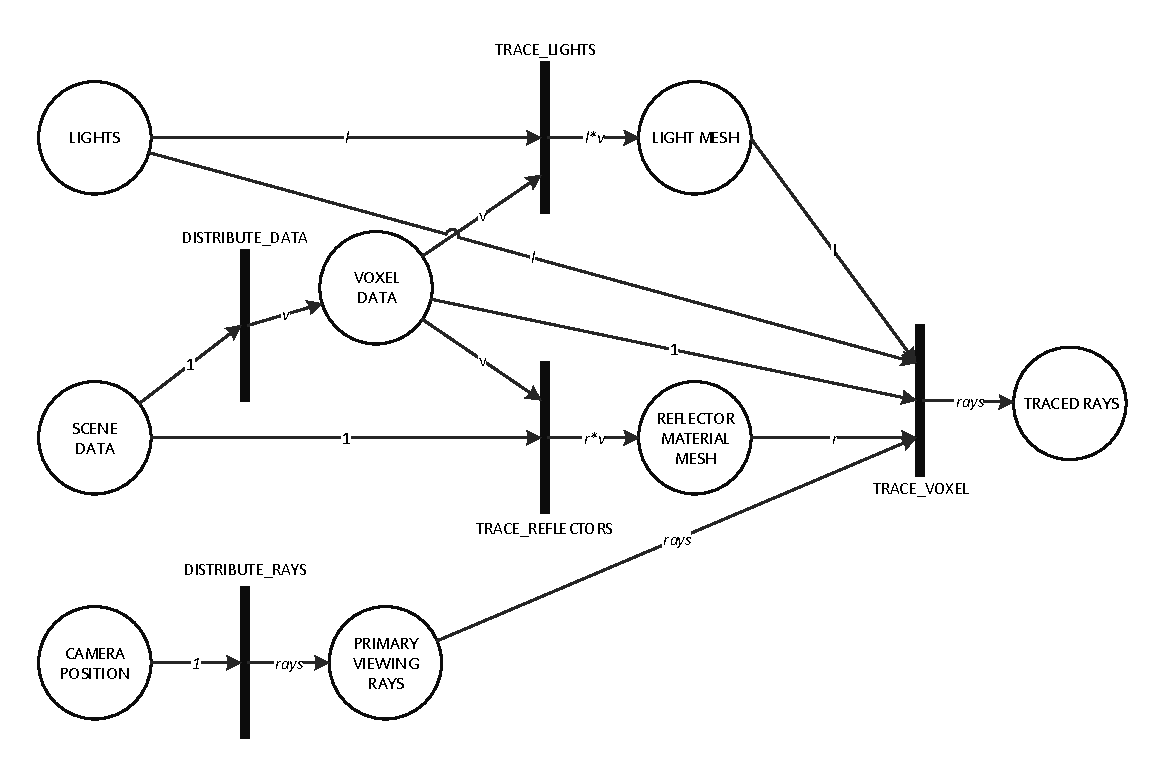
\includegraphics[width=\linewidth]{drawings/Design.pdf}
\caption{Proposed Design Petri Net}
\label{fig:design}
\end{figure}

\subsection{Inputs}
The required inputs for the ray tracer are lighting, camera and scene object 
properties.  There will be a single scene with potentially many lights.  
Additionally many camera positions can be traced, but each pass through 
\emph{traced rays} will use a single camera position.  The labels on the arcs 
indicate the quantity relationships.

\begin{figure}[!htb]
\minipage{0.4\textwidth}
\begin{algorithm}
DISTRIBUTE_DATA(scene, voxels)
  in:  the scene to be traced
       voxels to split the scene into
  out: filled voxel subsets of scene
  for all voxel in voxels do
    for all geometric_shape in scene do
      if geometric_shape is in voxel then
        voxel.data.add(geometric_shape)
      end if
    end for
  end for
return voxels
\end{algorithm}

Distribute data
\endminipage\hfill
\caption{Ray tracer pseudo code}
\label{fig:ray_tracing_1}
\end{figure}

\subsection{Distribute data}
The transition, \textbf{distribute\_data} takes a \emph{scene} and the 
\emph{voxels} and fills them with subsets of the scenes data, see 
figure~\ref{fig:ray_tracing_1}.

\subsection{Distribute rays}
The transition, \textbf{distribute\_rays}, takes either camera properties as 
input or information regarding refracted rays from the output of a voxel 
computation and produces a set of viewing rays.  \emph{Primary Viewing Rays} are 
the resulting computed sets.

\begin{figure}[!htb]
\minipage{0.4\textwidth}
\begin{algorithm}
TRACE_LIGHTS(lights, voxels) 
  in:  lights in the scene
       voxel data
  out: light mesh for each voxel
  for all light in lights do
    light_mesh = false;
    for all voxel in voxels do 
      if not light_mesh then
        light_mesh = 
          COMPUTE_MESH(light, voxel)
      else
        light_mesh = 
          PROPIGATE_MESH(light_mesh, 
                       light, voxel)
      end if
      light_mesh_ = COPY(light_mesh)
      voxel.light_meshes.add(light_mesh_)
    end for
  end for
return voxels


.
\end{algorithm}

(a) Trace lights

\endminipage\hfill
\minipage{0.4\textwidth}
\begin{algorithm}
TRACE_REFLECTORS(scene, voxels) 
  in:  scene to be traced
       voxel data
  out: material mesh for each reflector
  material_meshes[,]
  for all objects in scene do
    material_mesh = false
    if object is reflector then
      for all voxel in voxels do 
        if not light_mesh then
          material_mesh = 
            COMPUTE_MESH(object, voxel)
        else
          material_mesh = 
            PROPIGATE_MESH(material_mesh, 
                         object, voxel)
        end if
      end for
      material_meshes.add(object, 
                         material_mesh)
    end if
  end for
return material_meshes
\end{algorithm}

(b) Trace reflectors

\endminipage\hfill
\caption{Ray tracer pseudo code}
\label{fig:ray_tracing_2}
\end{figure}

\subsection{Trace lights}
The transition, \textbf{trace\_lights} fires for each light in the domain and
uses the voxel data sets to produce a light mesh for each light for each
voxel.  \emph{Light Mesh} is the resulting mesh.  Pseudo code can be found in 
figure~\ref{fig:ray_tracing_2} a.

\subsection{Trace reflectors}
The transition, \textbf{trace\_reflectors} fires once for each scene and 
produces a material mesh for every reflector in the scene for each voxel.  
\emph{Reflector Material Mesh} is the resulting mesh.  The pseudo code for trace 
reflectors is similar to the pseudo code for trace lights and is presented in
 figure~\ref{fig:ray_tracing_2} b.

\subsection{Trace voxel}
The transition, \textbf{trace\_voxel} fires once for each voxel and produces a 
copy of the viewing rays with computed color information.  \emph{Traced Rays} 
are the resulting rays.  This transition uses the light meshes created for 
its voxel along with the material meshes.  It will also need the viewing 
rays and the lights.  Pseudo code for trace voxel can be found in 
figure~\ref{fig:ray_caster}.  Pseudo code for the helper method 
\textbf{compute\_color} is included in Section~\ref{sec:implementation}.


\begin{figure}[!htb]
\minipage{0.45\textwidth}
  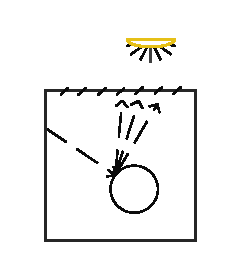
\includegraphics[width=6cm]{drawings/Case_1.pdf}
  
  (a) Light rays with no obstruction; handled by light mesh
  
  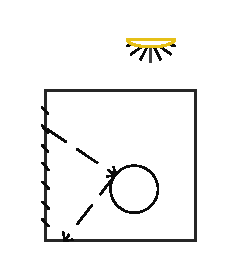
\includegraphics[width=6cm]{drawings/Case_3.pdf}
  
  (c) Reflected rays; handled by material mesh
  
\endminipage\hfill
\minipage{0.45\textwidth}
  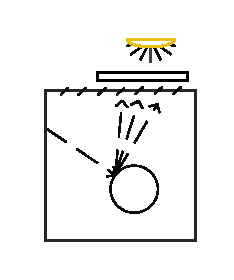
\includegraphics[width=6cm]{drawings/Case_2.pdf}
  
  (b) Light rays with obstruction; handled by light mesh
  
  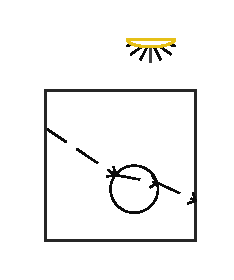
\includegraphics[width=6cm]{drawings/Case_4.pdf}
  
  (d) Refracted rays; handled by restart
  
\endminipage
\caption{Ray tracing algorithm cases}
\label{fig:use-cases}
\end{figure}

The algorithm presented here will handle ray casting as well as ray tracing for
scenes with multiple light sources as well as materials with reflection and
refraction material types.  The light mesh implementation can be found in 
section~\ref{sec:implementation}.  Additional detials on material meshse and the 
restart technique proposed for refracted rays can be found in section
~\ref{sec:future-work}.  A summary of the use cases supported are outlined in
figure~\ref{fig:use-cases}.
















